% Integrated appendices. The manuscript switches to one column before input.
\appendices

\section{Feature Contract, Temporal Evidence, and Outcome Definitions}
\label{app:features}

The primary \texttt{admission\_safe\_v1} contract contains 89 measured variables and two row-wise missingness indicators generated inside each training fold. The phrase ``admission stage'' follows the source data dictionary: columns 2--112, except the explicitly interval-defined columns 93--95 and 100--105, are documented as usable at admission. It does not imply that every field preceded all treatment decisions. In particular, seven fibrinolysis fields are retained because the source dictionary assigns them to the admission block, but the dataset lacks treatment timestamps. The estimand is therefore prediction from source-dictionary-defined admission-stage information, not a strict pretreatment model.

\begin{table}[ht]
\centering
\caption{Evidence boundary for variables requiring special temporal interpretation.}
\label{tab:app_temporal_evidence}
\small
\begin{tabular}{p{0.24\textwidth}p{0.18\textwidth}p{0.48\textwidth}}
\toprule
Variable group & Primary handling & Evidence boundary \\
\midrule
\texttt{fibr\_ter\_01--03,05--08} & Included (7 fields) & Located in the source dictionary's admission-use block; treatment timestamps are unavailable, so these variables cannot be guaranteed to precede therapy. \\
Initial laboratory values & Included & Documented as initial measurements; exact sampling time relative to immediate treatment is unavailable. \\
Admission manifestations and ECG findings & Included & Available in the admission record, but some manifestations may overlap clinically with later coded hospitalization outcomes. \\
Hospital-interval counts & Excluded from primary analysis & Added only in the 24-, 48-, and 72-hour accumulated-information sensitivity analyses. \\
Timing-ambiguous inpatient treatments & Excluded from primary analysis & Eleven treatment variables without a sufficiently clear admission-time definition were excluded. \\
\bottomrule
\end{tabular}
\end{table}

\scriptsize
\begin{longtable}{rlccccc}
\caption{Complete feature-contract membership. The two variables ending in MISSING are row-wise indicators whose definition is fixed but whose imputation/scaling objects are fitted only on training rows.}\label{tab:supp_features}\\
\toprule
No. & Variable & Admission & 24 h & 48 h & 72 h & Retrospective \\
\midrule
\endfirsthead
\multicolumn{7}{c}{\tablename\ \thetable\ (continued)}\\
\toprule
No. & Variable & Admission & 24 h & 48 h & 72 h & Retrospective \\
\midrule
\endhead
\midrule
\multicolumn{7}{r}{Continued on next page}\\
\endfoot
\bottomrule
\endlastfoot
1 & AGE & Yes & Yes & Yes & Yes & Yes \\
2 & SEX & Yes & Yes & Yes & Yes & Yes \\
3 & INF\_ANAM & Yes & Yes & Yes & Yes & Yes \\
4 & STENOK\_AN & Yes & Yes & Yes & Yes & Yes \\
5 & FK\_STENOK & Yes & Yes & Yes & Yes & Yes \\
6 & IBS\_POST & Yes & Yes & Yes & Yes & Yes \\
7 & GB & Yes & Yes & Yes & Yes & Yes \\
8 & SIM\_GIPERT & Yes & Yes & Yes & Yes & Yes \\
9 & DLIT\_AG & Yes & Yes & Yes & Yes & Yes \\
10 & ZSN\_A & Yes & Yes & Yes & Yes & Yes \\
11 & nr\_11 & Yes & Yes & Yes & Yes & Yes \\
12 & nr\_01 & Yes & Yes & Yes & Yes & Yes \\
13 & nr\_02 & Yes & Yes & Yes & Yes & Yes \\
14 & nr\_03 & Yes & Yes & Yes & Yes & Yes \\
15 & nr\_04 & Yes & Yes & Yes & Yes & Yes \\
16 & nr\_07 & Yes & Yes & Yes & Yes & Yes \\
17 & nr\_08 & Yes & Yes & Yes & Yes & Yes \\
18 & np\_01 & Yes & Yes & Yes & Yes & Yes \\
19 & np\_04 & Yes & Yes & Yes & Yes & Yes \\
20 & np\_05 & Yes & Yes & Yes & Yes & Yes \\
21 & np\_07 & Yes & Yes & Yes & Yes & Yes \\
22 & np\_08 & Yes & Yes & Yes & Yes & Yes \\
23 & np\_09 & Yes & Yes & Yes & Yes & Yes \\
24 & np\_10 & Yes & Yes & Yes & Yes & Yes \\
25 & endocr\_01 & Yes & Yes & Yes & Yes & Yes \\
26 & endocr\_02 & Yes & Yes & Yes & Yes & Yes \\
27 & endocr\_03 & Yes & Yes & Yes & Yes & Yes \\
28 & zab\_leg\_01 & Yes & Yes & Yes & Yes & Yes \\
29 & zab\_leg\_02 & Yes & Yes & Yes & Yes & Yes \\
30 & zab\_leg\_03 & Yes & Yes & Yes & Yes & Yes \\
31 & zab\_leg\_04 & Yes & Yes & Yes & Yes & Yes \\
32 & zab\_leg\_06 & Yes & Yes & Yes & Yes & Yes \\
33 & S\_AD\_KBRIG & Yes & Yes & Yes & Yes & Yes \\
34 & D\_AD\_KBRIG & Yes & Yes & Yes & Yes & Yes \\
35 & S\_AD\_ORIT & Yes & Yes & Yes & Yes & Yes \\
36 & D\_AD\_ORIT & Yes & Yes & Yes & Yes & Yes \\
37 & O\_L\_POST & Yes & Yes & Yes & Yes & Yes \\
38 & K\_SH\_POST & Yes & Yes & Yes & Yes & Yes \\
39 & MP\_TP\_POST & Yes & Yes & Yes & Yes & Yes \\
40 & SVT\_POST & Yes & Yes & Yes & Yes & Yes \\
41 & GT\_POST & Yes & Yes & Yes & Yes & Yes \\
42 & FIB\_G\_POST & Yes & Yes & Yes & Yes & Yes \\
43 & ant\_im & Yes & Yes & Yes & Yes & Yes \\
44 & lat\_im & Yes & Yes & Yes & Yes & Yes \\
45 & inf\_im & Yes & Yes & Yes & Yes & Yes \\
46 & post\_im & Yes & Yes & Yes & Yes & Yes \\
47 & IM\_PG\_P & Yes & Yes & Yes & Yes & Yes \\
48 & ritm\_ecg\_p\_01 & Yes & Yes & Yes & Yes & Yes \\
49 & ritm\_ecg\_p\_02 & Yes & Yes & Yes & Yes & Yes \\
50 & ritm\_ecg\_p\_04 & Yes & Yes & Yes & Yes & Yes \\
51 & ritm\_ecg\_p\_06 & Yes & Yes & Yes & Yes & Yes \\
52 & ritm\_ecg\_p\_07 & Yes & Yes & Yes & Yes & Yes \\
53 & ritm\_ecg\_p\_08 & Yes & Yes & Yes & Yes & Yes \\
54 & n\_r\_ecg\_p\_01 & Yes & Yes & Yes & Yes & Yes \\
55 & n\_r\_ecg\_p\_02 & Yes & Yes & Yes & Yes & Yes \\
56 & n\_r\_ecg\_p\_03 & Yes & Yes & Yes & Yes & Yes \\
57 & n\_r\_ecg\_p\_04 & Yes & Yes & Yes & Yes & Yes \\
58 & n\_r\_ecg\_p\_05 & Yes & Yes & Yes & Yes & Yes \\
59 & n\_r\_ecg\_p\_06 & Yes & Yes & Yes & Yes & Yes \\
60 & n\_r\_ecg\_p\_08 & Yes & Yes & Yes & Yes & Yes \\
61 & n\_r\_ecg\_p\_09 & Yes & Yes & Yes & Yes & Yes \\
62 & n\_r\_ecg\_p\_10 & Yes & Yes & Yes & Yes & Yes \\
63 & n\_p\_ecg\_p\_01 & Yes & Yes & Yes & Yes & Yes \\
64 & n\_p\_ecg\_p\_03 & Yes & Yes & Yes & Yes & Yes \\
65 & n\_p\_ecg\_p\_04 & Yes & Yes & Yes & Yes & Yes \\
66 & n\_p\_ecg\_p\_05 & Yes & Yes & Yes & Yes & Yes \\
67 & n\_p\_ecg\_p\_06 & Yes & Yes & Yes & Yes & Yes \\
68 & n\_p\_ecg\_p\_07 & Yes & Yes & Yes & Yes & Yes \\
69 & n\_p\_ecg\_p\_08 & Yes & Yes & Yes & Yes & Yes \\
70 & n\_p\_ecg\_p\_09 & Yes & Yes & Yes & Yes & Yes \\
71 & n\_p\_ecg\_p\_10 & Yes & Yes & Yes & Yes & Yes \\
72 & n\_p\_ecg\_p\_11 & Yes & Yes & Yes & Yes & Yes \\
73 & n\_p\_ecg\_p\_12 & Yes & Yes & Yes & Yes & Yes \\
74 & fibr\_ter\_01 & Yes & Yes & Yes & Yes & Yes \\
75 & fibr\_ter\_02 & Yes & Yes & Yes & Yes & Yes \\
76 & fibr\_ter\_03 & Yes & Yes & Yes & Yes & Yes \\
77 & fibr\_ter\_05 & Yes & Yes & Yes & Yes & Yes \\
78 & fibr\_ter\_06 & Yes & Yes & Yes & Yes & Yes \\
79 & fibr\_ter\_07 & Yes & Yes & Yes & Yes & Yes \\
80 & fibr\_ter\_08 & Yes & Yes & Yes & Yes & Yes \\
81 & GIPO\_K & Yes & Yes & Yes & Yes & Yes \\
82 & K\_BLOOD & Yes & Yes & Yes & Yes & Yes \\
83 & GIPER\_NA & Yes & Yes & Yes & Yes & Yes \\
84 & NA\_BLOOD & Yes & Yes & Yes & Yes & Yes \\
85 & ALT\_BLOOD & Yes & Yes & Yes & Yes & Yes \\
86 & AST\_BLOOD & Yes & Yes & Yes & Yes & Yes \\
87 & L\_BLOOD & Yes & Yes & Yes & Yes & Yes \\
88 & ROE & Yes & Yes & Yes & Yes & Yes \\
89 & TIME\_B\_S & Yes & Yes & Yes & Yes & Yes \\
90 & R\_AB\_1\_n & No & Yes & Yes & Yes & Yes \\
91 & R\_AB\_2\_n & No & No & Yes & Yes & Yes \\
92 & R\_AB\_3\_n & No & No & No & Yes & Yes \\
93 & NA\_KB & No & No & No & No & Yes \\
94 & NOT\_NA\_KB & No & No & No & No & Yes \\
95 & LID\_KB & No & No & No & No & Yes \\
96 & NITR\_S & No & No & No & No & Yes \\
97 & NA\_R\_1\_n & No & Yes & Yes & Yes & Yes \\
98 & NA\_R\_2\_n & No & No & Yes & Yes & Yes \\
99 & NA\_R\_3\_n & No & No & No & Yes & Yes \\
100 & NOT\_NA\_1\_n & No & Yes & Yes & Yes & Yes \\
101 & NOT\_NA\_2\_n & No & No & Yes & Yes & Yes \\
102 & NOT\_NA\_3\_n & No & No & No & Yes & Yes \\
103 & LID\_S\_n & No & No & No & No & Yes \\
104 & B\_BLOK\_S\_n & No & No & No & No & Yes \\
105 & ANT\_CA\_S\_n & No & No & No & No & Yes \\
106 & GEPAR\_S\_n & No & No & No & No & Yes \\
107 & ASP\_S\_n & No & No & No & No & Yes \\
108 & TIKL\_S\_n & No & No & No & No & Yes \\
109 & TRENT\_S\_n & No & No & No & No & Yes \\
110 & S\_AD\_KBRIG\_MISSING & Yes & Yes & Yes & Yes & Yes \\
111 & D\_AD\_KBRIG\_MISSING & Yes & Yes & Yes & Yes & Yes \\
\end{longtable}


The first 11 endpoints are binary source-coded hospitalization outcomes. The lethal field is converted to a binary endpoint as any nonzero coded lethal cause. No onset timestamps are available; hence prevalent manifestations and incident complications cannot always be separated.
\tiny
\begin{longtable}{lllp{0.22\textwidth}p{0.32\textwidth}}
\caption{Operational outcome definitions and interpretation boundaries from the source data dictionary.}\label{tab:supp_outcomes}\\
\toprule
Source field & Clinical label & Positive code & Operational target & Timing/interpretation caveat \\
\midrule
\endfirsthead
\multicolumn{5}{c}{\tablename\ \thetable\ (continued)}\\
\toprule
Source field & Clinical label & Positive code & Operational target & Timing/interpretation caveat \\
\midrule
\endhead
\midrule
\multicolumn{5}{r}{Continued on next page}\\
\endfoot
\bottomrule
\endlastfoot
FIBR\_PREDS & Atrial fibrillation & 1 & Recorded hospitalization complication & No onset timestamp; prevalent and incident events cannot be separated \\
PREDS\_TAH & Supraventricular tachycardia & 1 & Recorded hospitalization complication & Rare endpoint; no onset timestamp \\
JELUD\_TAH & Ventricular tachycardia & 1 & Recorded hospitalization complication & No onset timestamp \\
FIBR\_JELUD & Ventricular fibrillation & 1 & Recorded hospitalization complication & No onset timestamp \\
A\_V\_BLOK & Third-degree AV block & 1 & Recorded hospitalization complication & No onset timestamp \\
OTEK\_LANC & Pulmonary edema & 1 & Recorded hospitalization complication & No onset timestamp; may overlap a lethal-cause code \\
RAZRIV & Myocardial rupture & 1 & Recorded hospitalization complication & No onset timestamp; may overlap a lethal-cause code \\
DRESSLER & Dressler syndrome & 1 & Recorded hospitalization complication & May manifest after the early inpatient window \\
ZSN & Chronic heart failure outcome & 1 & Recorded hospitalization complication & Distinct field from baseline HF history but clinically overlapping; no onset timestamp \\
REC\_IM & Recurrent myocardial infarction & 1 & Recorded hospitalization complication & No onset timestamp \\
P\_IM\_STEN & Post-infarction angina & 1 & Recorded hospitalization complication & May manifest beyond the earliest observation window \\
LET\_IS & Fatal outcome & 1--7 & Any nonzero coded lethal cause & Cause code, not a time-to-event field; zero means no coded lethal cause \\
\end{longtable}


\section{Nested Validation, Fold Assignment, and Data-Use Audit}
\label{app:validation}

Five repeats of five outer folds produce one out-of-fold (OOF) probability for each patient in each repeat. Four inner folds determine CatBoost iterations, neural training epochs, the TabPFN-3 feature subset, and ensemble weights. Imputation, standardization, feature selection, class weighting, stopping decisions, and ensemble weights are fitted without access to the outer test fold. The final metric is computed after averaging the five OOF probabilities for each patient; it is not the mean of five separately calculated performance metrics.

\scriptsize
\begin{longtable}{rrrrrr}
\caption{Outer-fold size and event-count audit. Full per-label membership is provided in the machine-readable assignment file.}\label{tab:supp_folds}\\
\toprule
Repeat & Fold & $n$ & Minimum label events & Maximum label events & Deaths \\
\midrule
\endfirsthead
\multicolumn{6}{c}{\tablename\ \thetable\ (continued)}\\
\toprule
Repeat & Fold & $n$ & Minimum label events & Maximum label events & Deaths \\
\midrule
\endhead
\midrule
\multicolumn{6}{r}{Continued on next page}\\
\endfoot
\bottomrule
\endlastfoot
1 & 1 & 340 & 4 & 79 & 54 \\
1 & 2 & 340 & 4 & 78 & 54 \\
1 & 3 & 340 & 4 & 79 & 54 \\
1 & 4 & 340 & 4 & 79 & 55 \\
1 & 5 & 340 & 4 & 79 & 54 \\
2 & 1 & 340 & 4 & 79 & 54 \\
2 & 2 & 340 & 4 & 79 & 55 \\
2 & 3 & 340 & 4 & 78 & 54 \\
2 & 4 & 340 & 4 & 79 & 54 \\
2 & 5 & 340 & 4 & 79 & 54 \\
3 & 1 & 340 & 4 & 79 & 54 \\
3 & 2 & 340 & 4 & 79 & 54 \\
3 & 3 & 340 & 4 & 78 & 55 \\
3 & 4 & 340 & 4 & 79 & 54 \\
3 & 5 & 340 & 4 & 79 & 54 \\
4 & 1 & 340 & 4 & 79 & 54 \\
4 & 2 & 340 & 4 & 79 & 55 \\
4 & 3 & 340 & 4 & 78 & 54 \\
4 & 4 & 340 & 4 & 79 & 54 \\
4 & 5 & 340 & 4 & 79 & 54 \\
5 & 1 & 340 & 5 & 78 & 54 \\
5 & 2 & 340 & 4 & 79 & 54 \\
5 & 3 & 340 & 4 & 79 & 54 \\
5 & 4 & 340 & 3 & 79 & 54 \\
5 & 5 & 340 & 4 & 79 & 55 \\
\end{longtable}


The public configuration records all hyperparameters. TabPFN results were produced with \texttt{tabpfn==8.0.1} and checkpoint \path{tabpfn-v3-classifier-v3_default.ckpt}. Its SHA-256 digest is
\begin{center}
\footnotesize\texttt{D0D865D54DFBC524\allowbreak F5703104BE906201\allowbreak 82DCA7E5FB2C16DE\allowbreak 72E9959EA18F3988}.
\end{center}
The package resolves this checkpoint through its supported model cache; the licensed weight file is not redistributed.

\section{Complete Internal Performance, Paired Inference, and Calibration}
\label{app:internal}

Model-specific point estimates use the saved mean repeated-OOF predictions. The 2,000 paired patient bootstrap samples provide conditional uncertainty intervals for these saved predictions; they do not propagate the additional uncertainty that would arise from repeating every preprocessing, fitting, feature-selection, and inner-validation operation within each bootstrap sample.

\input{paper/generated_r1/supp_internal_models.tex}
\tiny
\begin{longtable}{llrrrrrrrl}
\caption{Per-label metrics for all internal models from mean repeated OOF predictions.}\label{tab:supp_internal_labels}\\
\toprule
Model & Label & Events & AUROC & AUPRC & Brier & ECE$_{10}$ & F1 & O:E & Calibration \\
\midrule
\endfirsthead
\multicolumn{10}{c}{\tablename\ \thetable\ (continued)}\\
\toprule
Model & Label & Events & AUROC & AUPRC & Brier & ECE$_{10}$ & F1 & O:E & Calibration \\
\midrule
\endhead
\midrule
\multicolumn{10}{r}{Continued on next page}\\
\endfoot
\bottomrule
\endlastfoot
BR--LR & FIBR\_PREDS & 170 & 0.723 & 0.253 & 0.183 & 0.274 & 0.299 & 0.268 & stable \\
BR--LR & PREDS\_TAH & 20 & 0.446 & 0.013 & 0.098 & 0.191 & 0.025 & 0.059 & unstable \\
BR--LR & JELUD\_TAH & 42 & 0.759 & 0.083 & 0.099 & 0.163 & 0.133 & 0.133 & stable \\
BR--LR & FIBR\_JELUD & 71 & 0.617 & 0.071 & 0.164 & 0.278 & 0.140 & 0.131 & stable \\
BR--LR & A\_V\_BLOK & 57 & 0.755 & 0.156 & 0.116 & 0.198 & 0.183 & 0.145 & stable \\
BR--LR & OTEK\_LANC & 159 & 0.649 & 0.154 & 0.207 & 0.306 & 0.226 & 0.234 & stable \\
BR--LR & RAZRIV & 54 & 0.761 & 0.121 & 0.123 & 0.193 & 0.152 & 0.142 & stable \\
BR--LR & DRESSLER & 75 & 0.646 & 0.071 & 0.178 & 0.294 & 0.112 & 0.130 & stable \\
BR--LR & ZSN & 394 & 0.672 & 0.352 & 0.223 & 0.220 & 0.437 & 0.513 & stable \\
BR--LR & REC\_IM & 159 & 0.630 & 0.156 & 0.210 & 0.314 & 0.223 & 0.229 & stable \\
BR--LR & P\_IM\_STEN & 148 & 0.678 & 0.155 & 0.205 & 0.308 & 0.238 & 0.220 & stable \\
BR--LR & LET\_IS & 271 & 0.842 & 0.577 & 0.148 & 0.183 & 0.525 & 0.466 & stable \\
BR--XGBoost & FIBR\_PREDS & 170 & 0.669 & 0.222 & 0.122 & 0.158 & 0.281 & 0.388 & stable \\
BR--XGBoost & PREDS\_TAH & 20 & 0.433 & 0.017 & 0.013 & 0.020 & 0.000 & 0.615 & unstable \\
BR--XGBoost & JELUD\_TAH & 42 & 0.678 & 0.051 & 0.030 & 0.038 & 0.000 & 0.414 & stable \\
BR--XGBoost & FIBR\_JELUD & 71 & 0.647 & 0.087 & 0.057 & 0.082 & 0.059 & 0.345 & stable \\
BR--XGBoost & A\_V\_BLOK & 57 & 0.674 & 0.102 & 0.041 & 0.056 & 0.120 & 0.403 & stable \\
BR--XGBoost & OTEK\_LANC & 159 & 0.604 & 0.123 & 0.124 & 0.151 & 0.114 & 0.386 & stable \\
BR--XGBoost & RAZRIV & 54 & 0.787 & 0.121 & 0.038 & 0.038 & 0.161 & 0.475 & stable \\
BR--XGBoost & DRESSLER & 75 & 0.581 & 0.068 & 0.063 & 0.099 & 0.038 & 0.315 & stable \\
BR--XGBoost & ZSN & 394 & 0.720 & 0.503 & 0.173 & 0.144 & 0.447 & 0.617 & stable \\
BR--XGBoost & REC\_IM & 159 & 0.609 & 0.141 & 0.122 & 0.158 & 0.167 & 0.373 & stable \\
BR--XGBoost & P\_IM\_STEN & 148 & 0.699 & 0.190 & 0.115 & 0.159 & 0.235 & 0.354 & stable \\
BR--XGBoost & LET\_IS & 271 & 0.852 & 0.591 & 0.112 & 0.106 & 0.554 & 0.601 & stable \\
BR--LightGBM & FIBR\_PREDS & 170 & 0.677 & 0.219 & 0.112 & 0.129 & 0.283 & 0.444 & stable \\
BR--LightGBM & PREDS\_TAH & 20 & 0.373 & 0.010 & 0.013 & 0.021 & 0.000 & 0.770 & unstable \\
BR--LightGBM & JELUD\_TAH & 42 & 0.711 & 0.067 & 0.027 & 0.026 & 0.042 & 0.551 & stable \\
BR--LightGBM & FIBR\_JELUD & 71 & 0.673 & 0.099 & 0.046 & 0.043 & 0.049 & 0.540 & stable \\
BR--LightGBM & A\_V\_BLOK & 57 & 0.677 & 0.119 & 0.036 & 0.037 & 0.110 & 0.577 & stable \\
BR--LightGBM & OTEK\_LANC & 159 & 0.617 & 0.127 & 0.108 & 0.099 & 0.112 & 0.487 & stable \\
BR--LightGBM & RAZRIV & 54 & 0.787 & 0.118 & 0.035 & 0.032 & 0.082 & 0.608 & stable \\
BR--LightGBM & DRESSLER & 75 & 0.610 & 0.069 & 0.051 & 0.059 & 0.000 & 0.480 & stable \\
BR--LightGBM & ZSN & 394 & 0.723 & 0.498 & 0.170 & 0.131 & 0.448 & 0.638 & stable \\
BR--LightGBM & REC\_IM & 159 & 0.622 & 0.148 & 0.105 & 0.109 & 0.121 & 0.472 & stable \\
BR--LightGBM & P\_IM\_STEN & 148 & 0.689 & 0.199 & 0.094 & 0.095 & 0.182 & 0.489 & stable \\
BR--LightGBM & LET\_IS & 271 & 0.859 & 0.611 & 0.104 & 0.086 & 0.574 & 0.651 & stable \\
BR--CatBoost & FIBR\_PREDS & 170 & 0.697 & 0.216 & 0.193 & 0.327 & 0.293 & 0.234 & stable \\
BR--CatBoost & PREDS\_TAH & 20 & 0.474 & 0.014 & 0.163 & 0.386 & 0.000 & 0.030 & unstable \\
BR--CatBoost & JELUD\_TAH & 42 & 0.666 & 0.055 & 0.121 & 0.304 & 0.075 & 0.075 & stable \\
BR--CatBoost & FIBR\_JELUD & 71 & 0.647 & 0.101 & 0.159 & 0.341 & 0.164 & 0.109 & stable \\
BR--CatBoost & A\_V\_BLOK & 57 & 0.724 & 0.108 & 0.157 & 0.349 & 0.221 & 0.088 & stable \\
BR--CatBoost & OTEK\_LANC & 159 & 0.639 & 0.154 & 0.206 & 0.350 & 0.199 & 0.211 & stable \\
BR--CatBoost & RAZRIV & 54 & 0.805 & 0.201 & 0.110 & 0.273 & 0.238 & 0.104 & stable \\
BR--CatBoost & DRESSLER & 75 & 0.587 & 0.072 & 0.194 & 0.388 & 0.119 & 0.102 & stable \\
BR--CatBoost & ZSN & 394 & 0.715 & 0.502 & 0.211 & 0.234 & 0.418 & 0.498 & stable \\
BR--CatBoost & REC\_IM & 159 & 0.620 & 0.149 & 0.217 & 0.364 & 0.220 & 0.204 & stable \\
BR--CatBoost & P\_IM\_STEN & 148 & 0.671 & 0.158 & 0.191 & 0.334 & 0.247 & 0.207 & stable \\
BR--CatBoost & LET\_IS & 271 & 0.848 & 0.604 & 0.131 & 0.179 & 0.540 & 0.472 & stable \\
ECC--LightGBM & FIBR\_PREDS & 170 & 0.690 & 0.245 & 0.085 & 0.027 & 0.065 & 1.245 & stable \\
ECC--LightGBM & PREDS\_TAH & 20 & 0.395 & 0.016 & 0.012 & 0.010 & 0.000 & 6.867 & unstable \\
ECC--LightGBM & JELUD\_TAH & 42 & 0.714 & 0.078 & 0.024 & 0.016 & 0.000 & 2.834 & stable \\
ECC--LightGBM & FIBR\_JELUD & 71 & 0.663 & 0.087 & 0.040 & 0.021 & 0.000 & 1.974 & stable \\
ECC--LightGBM & A\_V\_BLOK & 57 & 0.715 & 0.110 & 0.032 & 0.017 & 0.000 & 2.060 & stable \\
ECC--LightGBM & OTEK\_LANC & 159 & 0.635 & 0.133 & 0.086 & 0.042 & 0.000 & 1.414 & stable \\
ECC--LightGBM & RAZRIV & 54 & 0.801 & 0.121 & 0.031 & 0.018 & 0.000 & 2.220 & stable \\
ECC--LightGBM & DRESSLER & 75 & 0.601 & 0.070 & 0.043 & 0.025 & 0.000 & 1.684 & stable \\
ECC--LightGBM & ZSN & 394 & 0.727 & 0.504 & 0.149 & 0.031 & 0.374 & 1.065 & stable \\
ECC--LightGBM & REC\_IM & 159 & 0.636 & 0.162 & 0.084 & 0.033 & 0.000 & 1.447 & stable \\
ECC--LightGBM & P\_IM\_STEN & 148 & 0.693 & 0.201 & 0.076 & 0.022 & 0.026 & 1.123 & stable \\
ECC--LightGBM & LET\_IS & 271 & 0.862 & 0.611 & 0.094 & 0.026 & 0.419 & 1.186 & stable \\
LP--RF & FIBR\_PREDS & 170 & 0.725 & 0.236 & 0.085 & 0.034 & 0.000 & 1.018 & stable \\
LP--RF & PREDS\_TAH & 20 & 0.505 & 0.026 & 0.012 & 0.005 & 0.000 & 1.020 & unstable \\
LP--RF & JELUD\_TAH & 42 & 0.754 & 0.081 & 0.024 & 0.011 & 0.000 & 1.039 & stable \\
LP--RF & FIBR\_JELUD & 71 & 0.712 & 0.138 & 0.039 & 0.016 & 0.000 & 1.031 & stable \\
LP--RF & A\_V\_BLOK & 57 & 0.733 & 0.127 & 0.032 & 0.016 & 0.000 & 1.023 & stable \\
LP--RF & OTEK\_LANC & 159 & 0.693 & 0.164 & 0.082 & 0.024 & 0.000 & 1.020 & stable \\
LP--RF & RAZRIV & 54 & 0.834 & 0.149 & 0.030 & 0.024 & 0.000 & 1.022 & stable \\
LP--RF & DRESSLER & 75 & 0.682 & 0.079 & 0.042 & 0.017 & 0.000 & 1.007 & stable \\
LP--RF & ZSN & 394 & 0.726 & 0.512 & 0.156 & 0.047 & 0.182 & 1.009 & stable \\
LP--RF & REC\_IM & 159 & 0.668 & 0.170 & 0.083 & 0.026 & 0.000 & 1.007 & stable \\
LP--RF & P\_IM\_STEN & 148 & 0.681 & 0.182 & 0.077 & 0.034 & 0.000 & 0.985 & stable \\
LP--RF & LET\_IS & 271 & 0.853 & 0.589 & 0.102 & 0.069 & 0.280 & 1.039 & stable \\
RAkELd--RF & FIBR\_PREDS & 170 & 0.727 & 0.248 & 0.084 & 0.029 & 0.000 & 1.015 & stable \\
RAkELd--RF & PREDS\_TAH & 20 & 0.528 & 0.076 & 0.011 & 0.007 & 0.000 & 1.018 & unstable \\
RAkELd--RF & JELUD\_TAH & 42 & 0.746 & 0.079 & 0.024 & 0.009 & 0.000 & 1.029 & stable \\
RAkELd--RF & FIBR\_JELUD & 71 & 0.691 & 0.133 & 0.039 & 0.018 & 0.000 & 1.032 & stable \\
RAkELd--RF & A\_V\_BLOK & 57 & 0.739 & 0.160 & 0.031 & 0.012 & 0.000 & 1.025 & stable \\
RAkELd--RF & OTEK\_LANC & 159 & 0.671 & 0.155 & 0.083 & 0.020 & 0.000 & 1.024 & stable \\
RAkELd--RF & RAZRIV & 54 & 0.811 & 0.146 & 0.030 & 0.019 & 0.000 & 1.023 & stable \\
RAkELd--RF & DRESSLER & 75 & 0.686 & 0.081 & 0.042 & 0.011 & 0.000 & 1.006 & stable \\
RAkELd--RF & ZSN & 394 & 0.727 & 0.513 & 0.155 & 0.039 & 0.261 & 1.013 & stable \\
RAkELd--RF & REC\_IM & 159 & 0.665 & 0.164 & 0.083 & 0.022 & 0.000 & 1.012 & stable \\
RAkELd--RF & P\_IM\_STEN & 148 & 0.662 & 0.167 & 0.077 & 0.018 & 0.000 & 0.993 & stable \\
RAkELd--RF & LET\_IS & 271 & 0.855 & 0.594 & 0.100 & 0.058 & 0.287 & 1.038 & stable \\
Shared MLP & FIBR\_PREDS & 170 & 0.716 & 0.217 & 0.198 & 0.320 & 0.286 & 0.238 & stable \\
Shared MLP & PREDS\_TAH & 20 & 0.493 & 0.013 & 0.105 & 0.255 & 0.019 & 0.044 & unstable \\
Shared MLP & JELUD\_TAH & 42 & 0.737 & 0.064 & 0.116 & 0.236 & 0.121 & 0.095 & stable \\
Shared MLP & FIBR\_JELUD & 71 & 0.676 & 0.095 & 0.175 & 0.331 & 0.145 & 0.112 & stable \\
Shared MLP & A\_V\_BLOK & 57 & 0.757 & 0.139 & 0.128 & 0.259 & 0.185 & 0.115 & stable \\
Shared MLP & OTEK\_LANC & 159 & 0.670 & 0.176 & 0.211 & 0.337 & 0.235 & 0.217 & stable \\
Shared MLP & RAZRIV & 54 & 0.835 & 0.158 & 0.108 & 0.205 & 0.168 & 0.134 & stable \\
Shared MLP & DRESSLER & 75 & 0.633 & 0.073 & 0.188 & 0.349 & 0.116 & 0.112 & stable \\
Shared MLP & ZSN & 394 & 0.681 & 0.363 & 0.227 & 0.245 & 0.453 & 0.486 & stable \\
Shared MLP & REC\_IM & 159 & 0.650 & 0.170 & 0.217 & 0.354 & 0.223 & 0.209 & stable \\
Shared MLP & P\_IM\_STEN & 148 & 0.666 & 0.140 & 0.211 & 0.345 & 0.221 & 0.201 & stable \\
Shared MLP & LET\_IS & 271 & 0.849 & 0.587 & 0.149 & 0.197 & 0.518 & 0.448 & stable \\
Multitask DNN & FIBR\_PREDS & 170 & 0.710 & 0.209 & 0.195 & 0.307 & 0.287 & 0.245 & stable \\
Multitask DNN & PREDS\_TAH & 20 & 0.456 & 0.012 & 0.107 & 0.266 & 0.011 & 0.042 & unstable \\
Multitask DNN & JELUD\_TAH & 42 & 0.727 & 0.061 & 0.123 & 0.251 & 0.116 & 0.089 & stable \\
Multitask DNN & FIBR\_JELUD & 71 & 0.676 & 0.087 & 0.171 & 0.319 & 0.145 & 0.116 & stable \\
Multitask DNN & A\_V\_BLOK & 57 & 0.755 & 0.146 & 0.130 & 0.255 & 0.197 & 0.116 & stable \\
Multitask DNN & OTEK\_LANC & 159 & 0.672 & 0.169 & 0.210 & 0.331 & 0.232 & 0.221 & stable \\
Multitask DNN & RAZRIV & 54 & 0.827 & 0.152 & 0.108 & 0.195 & 0.176 & 0.140 & stable \\
Multitask DNN & DRESSLER & 75 & 0.621 & 0.070 & 0.192 & 0.350 & 0.099 & 0.112 & stable \\
Multitask DNN & ZSN & 394 & 0.697 & 0.378 & 0.219 & 0.231 & 0.457 & 0.501 & stable \\
Multitask DNN & REC\_IM & 159 & 0.641 & 0.168 & 0.214 & 0.345 & 0.229 & 0.213 & stable \\
Multitask DNN & P\_IM\_STEN & 148 & 0.670 & 0.142 & 0.210 & 0.334 & 0.224 & 0.207 & stable \\
Multitask DNN & LET\_IS & 271 & 0.844 & 0.588 & 0.152 & 0.195 & 0.523 & 0.450 & stable \\
TabPFN-3 & FIBR\_PREDS & 170 & 0.732 & 0.264 & 0.083 & 0.015 & 0.044 & 1.180 & stable \\
TabPFN-3 & PREDS\_TAH & 20 & 0.409 & 0.073 & 0.011 & 0.007 & 0.000 & 1.404 & unstable \\
TabPFN-3 & JELUD\_TAH & 42 & 0.753 & 0.072 & 0.024 & 0.009 & 0.000 & 1.396 & stable \\
TabPFN-3 & FIBR\_JELUD & 71 & 0.672 & 0.088 & 0.039 & 0.015 & 0.000 & 1.362 & stable \\
TabPFN-3 & A\_V\_BLOK & 57 & 0.794 & 0.172 & 0.030 & 0.010 & 0.000 & 1.298 & stable \\
TabPFN-3 & OTEK\_LANC & 159 & 0.678 & 0.165 & 0.082 & 0.021 & 0.000 & 1.217 & stable \\
TabPFN-3 & RAZRIV & 54 & 0.804 & 0.144 & 0.029 & 0.010 & 0.000 & 1.309 & stable \\
TabPFN-3 & DRESSLER & 75 & 0.592 & 0.073 & 0.042 & 0.017 & 0.000 & 1.336 & stable \\
TabPFN-3 & ZSN & 394 & 0.731 & 0.510 & 0.146 & 0.021 & 0.361 & 1.079 & stable \\
TabPFN-3 & REC\_IM & 159 & 0.621 & 0.145 & 0.084 & 0.023 & 0.000 & 1.231 & stable \\
TabPFN-3 & P\_IM\_STEN & 148 & 0.675 & 0.164 & 0.077 & 0.020 & 0.000 & 1.220 & stable \\
TabPFN-3 & LET\_IS & 271 & 0.873 & 0.624 & 0.091 & 0.015 & 0.489 & 1.099 & stable \\
LP--RF--TabPFN-3 (equal) & FIBR\_PREDS & 170 & 0.741 & 0.264 & 0.083 & 0.023 & 0.000 & 1.093 & stable \\
LP--RF--TabPFN-3 (equal) & PREDS\_TAH & 20 & 0.499 & 0.086 & 0.011 & 0.007 & 0.000 & 1.182 & unstable \\
LP--RF--TabPFN-3 (equal) & JELUD\_TAH & 42 & 0.774 & 0.079 & 0.024 & 0.010 & 0.000 & 1.191 & stable \\
LP--RF--TabPFN-3 (equal) & FIBR\_JELUD & 71 & 0.701 & 0.107 & 0.039 & 0.015 & 0.000 & 1.173 & stable \\
LP--RF--TabPFN-3 (equal) & A\_V\_BLOK & 57 & 0.788 & 0.175 & 0.031 & 0.013 & 0.000 & 1.144 & stable \\
LP--RF--TabPFN-3 (equal) & OTEK\_LANC & 159 & 0.689 & 0.170 & 0.082 & 0.023 & 0.000 & 1.110 & stable \\
LP--RF--TabPFN-3 (equal) & RAZRIV & 54 & 0.822 & 0.148 & 0.029 & 0.016 & 0.000 & 1.148 & stable \\
LP--RF--TabPFN-3 (equal) & DRESSLER & 75 & 0.667 & 0.085 & 0.042 & 0.011 & 0.000 & 1.148 & stable \\
LP--RF--TabPFN-3 (equal) & ZSN & 394 & 0.737 & 0.518 & 0.148 & 0.036 & 0.362 & 1.043 & stable \\
LP--RF--TabPFN-3 (equal) & REC\_IM & 159 & 0.653 & 0.162 & 0.083 & 0.030 & 0.000 & 1.108 & stable \\
LP--RF--TabPFN-3 (equal) & P\_IM\_STEN & 148 & 0.687 & 0.177 & 0.077 & 0.024 & 0.000 & 1.090 & stable \\
LP--RF--TabPFN-3 (equal) & LET\_IS & 271 & 0.870 & 0.627 & 0.094 & 0.043 & 0.350 & 1.068 & stable \\
LP--RF--TabPFN-3 (inner-OOF weighted) & FIBR\_PREDS & 170 & 0.741 & 0.264 & 0.083 & 0.022 & 0.000 & 1.094 & stable \\
LP--RF--TabPFN-3 (inner-OOF weighted) & PREDS\_TAH & 20 & 0.500 & 0.086 & 0.011 & 0.007 & 0.000 & 1.177 & unstable \\
LP--RF--TabPFN-3 (inner-OOF weighted) & JELUD\_TAH & 42 & 0.774 & 0.078 & 0.024 & 0.010 & 0.000 & 1.194 & stable \\
LP--RF--TabPFN-3 (inner-OOF weighted) & FIBR\_JELUD & 71 & 0.700 & 0.107 & 0.039 & 0.014 & 0.000 & 1.171 & stable \\
LP--RF--TabPFN-3 (inner-OOF weighted) & A\_V\_BLOK & 57 & 0.788 & 0.173 & 0.031 & 0.014 & 0.000 & 1.149 & stable \\
LP--RF--TabPFN-3 (inner-OOF weighted) & OTEK\_LANC & 159 & 0.689 & 0.170 & 0.082 & 0.023 & 0.000 & 1.109 & stable \\
LP--RF--TabPFN-3 (inner-OOF weighted) & RAZRIV & 54 & 0.823 & 0.149 & 0.029 & 0.016 & 0.000 & 1.147 & stable \\
LP--RF--TabPFN-3 (inner-OOF weighted) & DRESSLER & 75 & 0.668 & 0.085 & 0.042 & 0.011 & 0.000 & 1.145 & stable \\
LP--RF--TabPFN-3 (inner-OOF weighted) & ZSN & 394 & 0.737 & 0.518 & 0.148 & 0.036 & 0.362 & 1.043 & stable \\
LP--RF--TabPFN-3 (inner-OOF weighted) & REC\_IM & 159 & 0.653 & 0.163 & 0.083 & 0.031 & 0.000 & 1.105 & stable \\
LP--RF--TabPFN-3 (inner-OOF weighted) & P\_IM\_STEN & 148 & 0.687 & 0.177 & 0.077 & 0.023 & 0.000 & 1.089 & stable \\
LP--RF--TabPFN-3 (inner-OOF weighted) & LET\_IS & 271 & 0.870 & 0.627 & 0.094 & 0.043 & 0.350 & 1.068 & stable \\
\end{longtable}

\tiny
\begin{longtable}{lrrrrrrr}
\caption{Sensitivity to the five outer-fold repetitions. SD is descriptive across the five complete repeated OOF prediction sets and is not the primary confidence interval.}\label{tab:supp_repeat_stability}\\
\toprule
Model & Macro-AUROC mean & SD & Range & Macro-AUPRC mean & SD & Brier mean & SD \\
\midrule
\endfirsthead
\multicolumn{8}{c}{\tablename\ \thetable\ (continued)}\\
\toprule
Model & Macro-AUROC mean & SD & Range & Macro-AUPRC mean & SD & Brier mean & SD \\
\midrule
\endhead
\midrule
\multicolumn{8}{r}{Continued on next page}\\
\endfoot
\bottomrule
\endlastfoot
BR--LR & 0.6744 & 0.0051 & 0.6693--0.6821 & 0.1745 & 0.0036 & 0.1705 & 0.0006 \\
BR--XGBoost & 0.6450 & 0.0089 & 0.6372--0.6593 & 0.1753 & 0.0038 & 0.0912 & 0.0004 \\
BR--LightGBM & 0.6525 & 0.0053 & 0.6448--0.6588 & 0.1789 & 0.0027 & 0.0815 & 0.0003 \\
BR--CatBoost & 0.6552 & 0.0069 & 0.6462--0.6637 & 0.1814 & 0.0063 & 0.1756 & 0.0057 \\
ECC--LightGBM & 0.6640 & 0.0065 & 0.6571--0.6718 & 0.1853 & 0.0023 & 0.0641 & 0.0002 \\
LP--RF & 0.6993 & 0.0052 & 0.6916--0.7057 & 0.1942 & 0.0035 & 0.0637 & 0.0001 \\
RAkELd--RF & 0.6938 & 0.0060 & 0.6863--0.7001 & 0.1966 & 0.0056 & 0.0634 & 0.0002 \\
Shared MLP & 0.6856 & 0.0050 & 0.6785--0.6925 & 0.1748 & 0.0027 & 0.1756 & 0.0025 \\
Multitask DNN & 0.6818 & 0.0039 & 0.6770--0.6875 & 0.1759 & 0.0054 & 0.1751 & 0.0036 \\
TabPFN-3 & 0.6905 & 0.0029 & 0.6877--0.6938 & 0.2045 & 0.0040 & 0.0618 & 0.0002 \\
LP--RF--TabPFN-3 (equal) & 0.7133 & 0.0049 & 0.7078--0.7201 & 0.2118 & 0.0039 & 0.0620 & 0.0001 \\
LP--RF--TabPFN-3 (inner-OOF weighted) & 0.7134 & 0.0049 & 0.7079--0.7202 & 0.2117 & 0.0038 & 0.0620 & 0.0001 \\
\end{longtable}

\tiny
\begin{longtable}{lrlrrrrll}
\caption{Per-label primary paired comparison: weighted ensemble minus TabPFN-3.}\label{tab:supp_primary_inference}\\
\toprule
Label & Events & Test & $\Delta$AUROC & 95\% CI & $p$ & BH $q$ & Reject & Stability \\
\midrule
\endfirsthead
\multicolumn{9}{c}{\tablename\ \thetable\ (continued)}\\
\toprule
Label & Events & Test & $\Delta$AUROC & 95\% CI & $p$ & BH $q$ & Reject & Stability \\
\midrule
\endhead
\midrule
\multicolumn{9}{r}{Continued on next page}\\
\endfoot
\bottomrule
\endlastfoot
FIBR\_PREDS & 170 & paired DeLong & 0.0086 & $-$0.0011--0.0183 & 0.0796 & 0.1365 & No & stable \\
PREDS\_TAH & 20 & paired permutation & 0.0908 & $-$0.0129--0.1974 & 0.2747 & 0.2996 & No & unstable \\
JELUD\_TAH & 42 & paired DeLong & 0.0204 & $-$0.0097--0.0515 & 0.1946 & 0.2335 & No & stable \\
FIBR\_JELUD & 71 & paired DeLong & 0.0286 & 0.0091--0.0480 & 0.0036 & 0.0143 & Yes & stable \\
A\_V\_BLOK & 57 & paired DeLong & $-$0.0054 & $-$0.0254--0.0171 & 0.6084 & 0.6084 & No & stable \\
OTEK\_LANC & 159 & paired DeLong & 0.0107 & 0.0014--0.0207 & 0.0287 & 0.0788 & No & stable \\
RAZRIV & 54 & paired DeLong & 0.0190 & 0.0003--0.0365 & 0.0328 & 0.0788 & No & stable \\
DRESSLER & 75 & paired DeLong & 0.0763 & 0.0396--0.1160 & 0.0001 & 0.0006 & Yes & stable \\
ZSN & 394 & paired DeLong & 0.0056 & $-$0.0008--0.0121 & 0.0927 & 0.1391 & No & stable \\
REC\_IM & 159 & paired DeLong & 0.0320 & 0.0182--0.0459 & 0.0000 & 0.0001 & Yes & stable \\
P\_IM\_STEN & 148 & paired DeLong & 0.0119 & $-$0.0006--0.0250 & 0.0705 & 0.1365 & No & stable \\
LET\_IS & 271 & paired DeLong & $-$0.0030 & $-$0.0075--0.0014 & 0.1803 & 0.2335 & No & stable \\
\end{longtable}

\tiny
\begin{longtable}{llrlrrrl}
\caption{Per-label calibration estimates and 95\% patient-bootstrap intervals for the primary models.}\label{tab:supp_calibration}\\
\toprule
Model & Label & Events & Metric & Estimate & CI low & CI high & Stability \\
\midrule
\endfirsthead
\multicolumn{8}{c}{\tablename\ \thetable\ (continued)}\\
\toprule
Model & Label & Events & Metric & Estimate & CI low & CI high & Stability \\
\midrule
\endhead
\midrule
\multicolumn{8}{r}{Continued on next page}\\
\endfoot
\bottomrule
\endlastfoot
LP--RF--TabPFN-3 (inner-OOF weighted) & FIBR\_PREDS & 170 & brier & 0.0832 & 0.0734 & 0.0937 & stable \\
LP--RF--TabPFN-3 (inner-OOF weighted) & FIBR\_PREDS & 170 & ece\_10 & 0.0220 & 0.0185 & 0.0399 & stable \\
LP--RF--TabPFN-3 (inner-OOF weighted) & FIBR\_PREDS & 170 & calibration\_intercept & 0.9665 & 0.4080 & 1.5343 & stable \\
LP--RF--TabPFN-3 (inner-OOF weighted) & FIBR\_PREDS & 170 & calibration\_slope & 1.4078 & 1.1698 & 1.6756 & stable \\
LP--RF--TabPFN-3 (inner-OOF weighted) & PREDS\_TAH & 20 & brier & 0.0115 & 0.0069 & 0.0167 & unstable \\
LP--RF--TabPFN-3 (inner-OOF weighted) & PREDS\_TAH & 20 & ece\_10 & 0.0074 & 0.0055 & 0.0136 & unstable \\
LP--RF--TabPFN-3 (inner-OOF weighted) & PREDS\_TAH & 20 & calibration\_intercept & 1.3068 & $-$9.0641 & 5.0223 & unstable \\
LP--RF--TabPFN-3 (inner-OOF weighted) & PREDS\_TAH & 20 & calibration\_slope & 1.2559 & $-$0.9394 & 2.1246 & unstable \\
LP--RF--TabPFN-3 (inner-OOF weighted) & JELUD\_TAH & 42 & brier & 0.0236 & 0.0170 & 0.0306 & stable \\
LP--RF--TabPFN-3 (inner-OOF weighted) & JELUD\_TAH & 42 & ece\_10 & 0.0097 & 0.0073 & 0.0195 & stable \\
LP--RF--TabPFN-3 (inner-OOF weighted) & JELUD\_TAH & 42 & calibration\_intercept & 1.7036 & 0.2572 & 3.1349 & stable \\
LP--RF--TabPFN-3 (inner-OOF weighted) & JELUD\_TAH & 42 & calibration\_slope & 1.4253 & 1.0506 & 1.8387 & stable \\
LP--RF--TabPFN-3 (inner-OOF weighted) & FIBR\_JELUD & 71 & brier & 0.0392 & 0.0312 & 0.0477 & stable \\
LP--RF--TabPFN-3 (inner-OOF weighted) & FIBR\_JELUD & 71 & ece\_10 & 0.0143 & 0.0114 & 0.0261 & stable \\
LP--RF--TabPFN-3 (inner-OOF weighted) & FIBR\_JELUD & 71 & calibration\_intercept & 2.0433 & 0.4491 & 3.6666 & stable \\
LP--RF--TabPFN-3 (inner-OOF weighted) & FIBR\_JELUD & 71 & calibration\_slope & 1.5976 & 1.1093 & 2.1413 & stable \\
LP--RF--TabPFN-3 (inner-OOF weighted) & A\_V\_BLOK & 57 & brier & 0.0305 & 0.0233 & 0.0382 & stable \\
LP--RF--TabPFN-3 (inner-OOF weighted) & A\_V\_BLOK & 57 & ece\_10 & 0.0140 & 0.0100 & 0.0234 & stable \\
LP--RF--TabPFN-3 (inner-OOF weighted) & A\_V\_BLOK & 57 & calibration\_intercept & 1.4925 & 0.4653 & 2.5587 & stable \\
LP--RF--TabPFN-3 (inner-OOF weighted) & A\_V\_BLOK & 57 & calibration\_slope & 1.4303 & 1.1136 & 1.7981 & stable \\
LP--RF--TabPFN-3 (inner-OOF weighted) & OTEK\_LANC & 159 & brier & 0.0821 & 0.0713 & 0.0929 & stable \\
LP--RF--TabPFN-3 (inner-OOF weighted) & OTEK\_LANC & 159 & ece\_10 & 0.0226 & 0.0163 & 0.0371 & stable \\
LP--RF--TabPFN-3 (inner-OOF weighted) & OTEK\_LANC & 159 & calibration\_intercept & 0.8275 & 0.0949 & 1.5927 & stable \\
LP--RF--TabPFN-3 (inner-OOF weighted) & OTEK\_LANC & 159 & calibration\_slope & 1.3159 & 1.0134 & 1.6757 & stable \\
LP--RF--TabPFN-3 (inner-OOF weighted) & RAZRIV & 54 & brier & 0.0293 & 0.0221 & 0.0374 & stable \\
LP--RF--TabPFN-3 (inner-OOF weighted) & RAZRIV & 54 & ece\_10 & 0.0164 & 0.0117 & 0.0262 & stable \\
LP--RF--TabPFN-3 (inner-OOF weighted) & RAZRIV & 54 & calibration\_intercept & 2.1294 & 0.9201 & 3.4741 & stable \\
LP--RF--TabPFN-3 (inner-OOF weighted) & RAZRIV & 54 & calibration\_slope & 1.6340 & 1.2656 & 2.0823 & stable \\
LP--RF--TabPFN-3 (inner-OOF weighted) & DRESSLER & 75 & brier & 0.0417 & 0.0334 & 0.0509 & stable \\
LP--RF--TabPFN-3 (inner-OOF weighted) & DRESSLER & 75 & ece\_10 & 0.0113 & 0.0099 & 0.0250 & stable \\
LP--RF--TabPFN-3 (inner-OOF weighted) & DRESSLER & 75 & calibration\_intercept & 2.1705 & 0.3628 & 4.0533 & stable \\
LP--RF--TabPFN-3 (inner-OOF weighted) & DRESSLER & 75 & calibration\_slope & 1.6494 & 1.0775 & 2.2644 & stable \\
LP--RF--TabPFN-3 (inner-OOF weighted) & ZSN & 394 & brier & 0.1475 & 0.1377 & 0.1585 & stable \\
LP--RF--TabPFN-3 (inner-OOF weighted) & ZSN & 394 & ece\_10 & 0.0361 & 0.0299 & 0.0582 & stable \\
LP--RF--TabPFN-3 (inner-OOF weighted) & ZSN & 394 & calibration\_intercept & 0.5755 & 0.3401 & 0.8470 & stable \\
LP--RF--TabPFN-3 (inner-OOF weighted) & ZSN & 394 & calibration\_slope & 1.4262 & 1.2557 & 1.6231 & stable \\
LP--RF--TabPFN-3 (inner-OOF weighted) & REC\_IM & 159 & brier & 0.0830 & 0.0716 & 0.0941 & stable \\
LP--RF--TabPFN-3 (inner-OOF weighted) & REC\_IM & 159 & ece\_10 & 0.0310 & 0.0234 & 0.0466 & stable \\
LP--RF--TabPFN-3 (inner-OOF weighted) & REC\_IM & 159 & calibration\_intercept & 1.3036 & 0.1128 & 2.5275 & stable \\
LP--RF--TabPFN-3 (inner-OOF weighted) & REC\_IM & 159 & calibration\_slope & 1.5171 & 1.0063 & 2.0714 & stable \\
LP--RF--TabPFN-3 (inner-OOF weighted) & P\_IM\_STEN & 148 & brier & 0.0771 & 0.0668 & 0.0882 & stable \\
LP--RF--TabPFN-3 (inner-OOF weighted) & P\_IM\_STEN & 148 & ece\_10 & 0.0225 & 0.0197 & 0.0409 & stable \\
LP--RF--TabPFN-3 (inner-OOF weighted) & P\_IM\_STEN & 148 & calibration\_intercept & 2.0646 & 0.8901 & 3.3704 & stable \\
LP--RF--TabPFN-3 (inner-OOF weighted) & P\_IM\_STEN & 148 & calibration\_slope & 1.8418 & 1.3463 & 2.4169 & stable \\
LP--RF--TabPFN-3 (inner-OOF weighted) & LET\_IS & 271 & brier & 0.0937 & 0.0849 & 0.1035 & stable \\
LP--RF--TabPFN-3 (inner-OOF weighted) & LET\_IS & 271 & ece\_10 & 0.0431 & 0.0333 & 0.0595 & stable \\
LP--RF--TabPFN-3 (inner-OOF weighted) & LET\_IS & 271 & calibration\_intercept & 0.8318 & 0.5327 & 1.1777 & stable \\
LP--RF--TabPFN-3 (inner-OOF weighted) & LET\_IS & 271 & calibration\_slope & 1.4955 & 1.3306 & 1.6892 & stable \\
TabPFN-3 & FIBR\_PREDS & 170 & brier & 0.0829 & 0.0722 & 0.0945 & stable \\
TabPFN-3 & FIBR\_PREDS & 170 & ece\_10 & 0.0154 & 0.0123 & 0.0339 & stable \\
TabPFN-3 & FIBR\_PREDS & 170 & calibration\_intercept & 0.0686 & $-$0.3533 & 0.5108 & stable \\
TabPFN-3 & FIBR\_PREDS & 170 & calibration\_slope & 0.9378 & 0.7593 & 1.1312 & stable \\
TabPFN-3 & PREDS\_TAH & 20 & brier & 0.0114 & 0.0068 & 0.0165 & unstable \\
TabPFN-3 & PREDS\_TAH & 20 & ece\_10 & 0.0072 & 0.0055 & 0.0138 & unstable \\
TabPFN-3 & PREDS\_TAH & 20 & calibration\_intercept & 1.0733 & $-$3.6072 & 4.6610 & unstable \\
TabPFN-3 & PREDS\_TAH & 20 & calibration\_slope & 1.1574 & 0.1696 & 1.9241 & unstable \\
TabPFN-3 & JELUD\_TAH & 42 & brier & 0.0237 & 0.0171 & 0.0306 & stable \\
TabPFN-3 & JELUD\_TAH & 42 & ece\_10 & 0.0091 & 0.0064 & 0.0179 & stable \\
TabPFN-3 & JELUD\_TAH & 42 & calibration\_intercept & 0.0481 & $-$1.1783 & 1.1510 & stable \\
TabPFN-3 & JELUD\_TAH & 42 & calibration\_slope & 0.9161 & 0.6198 & 1.2240 & stable \\
TabPFN-3 & FIBR\_JELUD & 71 & brier & 0.0395 & 0.0306 & 0.0484 & stable \\
TabPFN-3 & FIBR\_JELUD & 71 & ece\_10 & 0.0154 & 0.0103 & 0.0270 & stable \\
TabPFN-3 & FIBR\_JELUD & 71 & calibration\_intercept & 0.2097 & $-$1.1913 & 1.4944 & stable \\
TabPFN-3 & FIBR\_JELUD & 71 & calibration\_slope & 0.9646 & 0.5630 & 1.3517 & stable \\
TabPFN-3 & A\_V\_BLOK & 57 & brier & 0.0302 & 0.0231 & 0.0374 & stable \\
TabPFN-3 & A\_V\_BLOK & 57 & ece\_10 & 0.0096 & 0.0071 & 0.0195 & stable \\
TabPFN-3 & A\_V\_BLOK & 57 & calibration\_intercept & 0.0431 & $-$0.6860 & 0.7841 & stable \\
TabPFN-3 & A\_V\_BLOK & 57 & calibration\_slope & 0.9174 & 0.7094 & 1.1551 & stable \\
TabPFN-3 & OTEK\_LANC & 159 & brier & 0.0825 & 0.0710 & 0.0932 & stable \\
TabPFN-3 & OTEK\_LANC & 159 & ece\_10 & 0.0205 & 0.0160 & 0.0380 & stable \\
TabPFN-3 & OTEK\_LANC & 159 & calibration\_intercept & 0.0796 & $-$0.5275 & 0.6725 & stable \\
TabPFN-3 & OTEK\_LANC & 159 & calibration\_slope & 0.9384 & 0.6972 & 1.1874 & stable \\
TabPFN-3 & RAZRIV & 54 & brier & 0.0293 & 0.0223 & 0.0366 & stable \\
TabPFN-3 & RAZRIV & 54 & ece\_10 & 0.0097 & 0.0068 & 0.0198 & stable \\
TabPFN-3 & RAZRIV & 54 & calibration\_intercept & 0.1292 & $-$0.8455 & 1.1166 & stable \\
TabPFN-3 & RAZRIV & 54 & calibration\_slope & 0.9476 & 0.6725 & 1.2713 & stable \\
TabPFN-3 & DRESSLER & 75 & brier & 0.0419 & 0.0334 & 0.0514 & stable \\
TabPFN-3 & DRESSLER & 75 & ece\_10 & 0.0174 & 0.0119 & 0.0290 & stable \\
TabPFN-3 & DRESSLER & 75 & calibration\_intercept & 0.1819 & $-$1.9226 & 1.7091 & stable \\
TabPFN-3 & DRESSLER & 75 & calibration\_slope & 0.9629 & 0.3588 & 1.4294 & stable \\
TabPFN-3 & ZSN & 394 & brier & 0.1458 & 0.1343 & 0.1573 & stable \\
TabPFN-3 & ZSN & 394 & ece\_10 & 0.0213 & 0.0198 & 0.0461 & stable \\
TabPFN-3 & ZSN & 394 & calibration\_intercept & 0.0514 & $-$0.1715 & 0.2983 & stable \\
TabPFN-3 & ZSN & 394 & calibration\_slope & 0.9465 & 0.8186 & 1.1006 & stable \\
TabPFN-3 & REC\_IM & 159 & brier & 0.0838 & 0.0728 & 0.0955 & stable \\
TabPFN-3 & REC\_IM & 159 & ece\_10 & 0.0228 & 0.0183 & 0.0401 & stable \\
TabPFN-3 & REC\_IM & 159 & calibration\_intercept & 0.3173 & $-$0.8179 & 1.4436 & stable \\
TabPFN-3 & REC\_IM & 159 & calibration\_slope & 1.0359 & 0.5967 & 1.5114 & stable \\
TabPFN-3 & P\_IM\_STEN & 148 & brier & 0.0772 & 0.0661 & 0.0887 & stable \\
TabPFN-3 & P\_IM\_STEN & 148 & ece\_10 & 0.0198 & 0.0154 & 0.0366 & stable \\
TabPFN-3 & P\_IM\_STEN & 148 & calibration\_intercept & 1.1289 & 0.1183 & 2.1077 & stable \\
TabPFN-3 & P\_IM\_STEN & 148 & calibration\_slope & 1.3707 & 0.9706 & 1.7842 & stable \\
TabPFN-3 & LET\_IS & 271 & brier & 0.0905 & 0.0798 & 0.0999 & stable \\
TabPFN-3 & LET\_IS & 271 & ece\_10 & 0.0151 & 0.0113 & 0.0323 & stable \\
TabPFN-3 & LET\_IS & 271 & calibration\_intercept & 0.1388 & $-$0.1033 & 0.3916 & stable \\
TabPFN-3 & LET\_IS & 271 & calibration\_slope & 0.9790 & 0.8611 & 1.1177 & stable \\
\end{longtable}


Calibration intercept and slope are estimated simultaneously from a logistic recalibration model. The unweighted BR-logistic sensitivity uses the identical 5$\times$5 outer folds and fold-local preprocessing, but sets \texttt{class\_weight=None}; it is reported only to examine the calibration cost of class weighting and does not alter the primary model ranking.
\begin{center}
\captionof{table}{Unweighted BR-logistic calibration sensitivity from the same mean repeated OOF predictions. This appendix analysis does not alter the primary model ranking.}\label{tab:app_unweighted_lr}
\resizebox{\textwidth}{!}{%
\begin{tabular}{lrrrrrrr}
\toprule
Model & Macro-AUROC & Macro-AUPRC & Brier & ECE$_{10}$ & Macro-F1 & Median intercept & Median slope \\
\midrule
BR--LR (unweighted) & 0.6936 & 0.1786 & 0.0653 & 0.0194 & 0.0736 & $-$0.886 & 0.669 \\
\bottomrule
\end{tabular}%
}
\end{center}


\begin{figure}[ht]
\centering
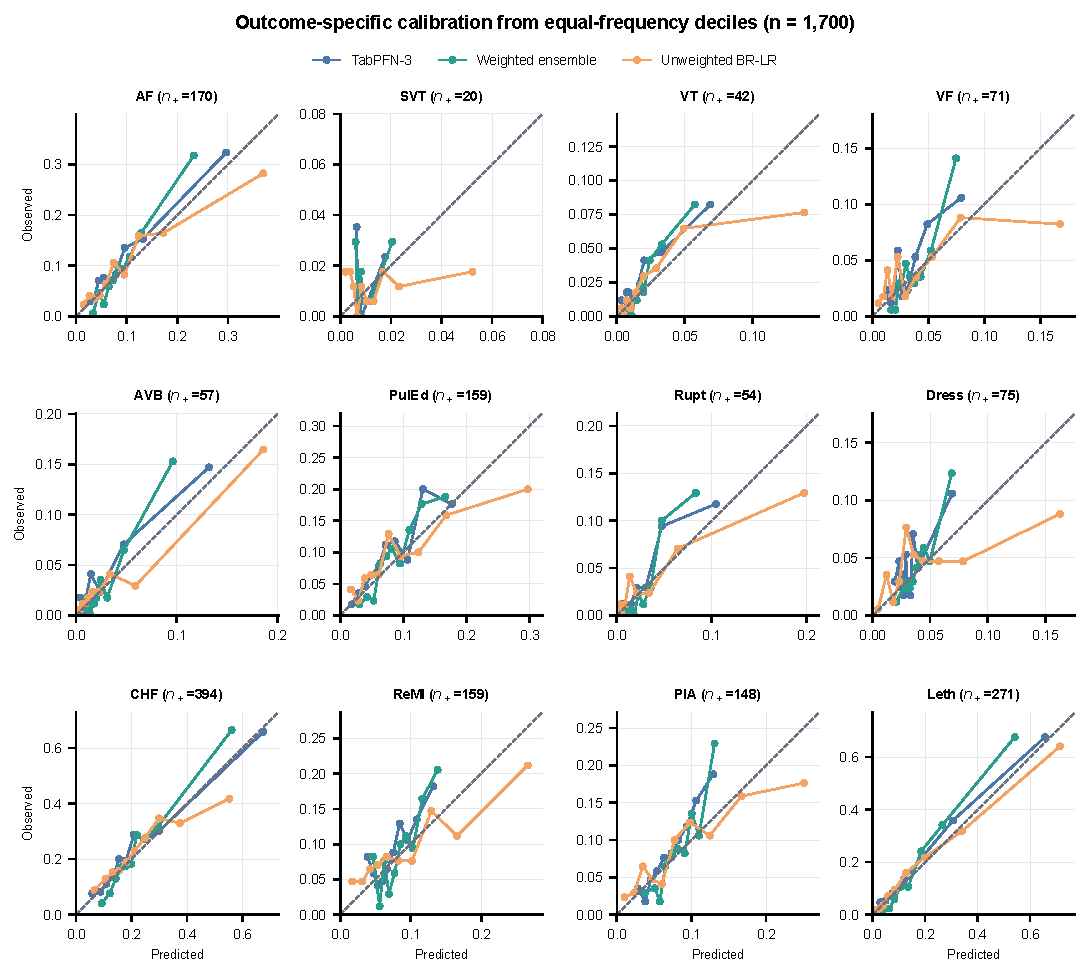
\includegraphics[width=0.96\textwidth,keepaspectratio]{figures/r1/fig_calibration_small_multiples.pdf}
\caption{Outcome-specific calibration for TabPFN-3, the inner-OOF-weighted ensemble, and unweighted BR-logistic regression. Each point represents an equal-frequency prediction decile for one outcome; the dashed diagonal denotes ideal calibration. Panel titles give the outcome abbreviation and positive count.}
\label{fig:app_calibration_small_multiples}
\end{figure}

\section{Ten-Seed, Eighteen-Configuration GCN Ablation}
\label{app:gcn}

The ablation compares optimization randomness across seeds 42--51 on one fixed train-validation-test partition. Within a seed, matched graph and no-graph variants share initialization, epoch-wise batch order, architecture, optimizer, and training protocol. These results do not establish model equivalence, causal effects of graph edges, or generalization across alternative partitions.
\tiny
\begin{longtable}{rllllrrr}
\caption{Complete 18-configuration GCN ablation for seeds 42--51.}\label{tab:supp_gcn_full}\\
\toprule
Seed & Graph & Head & Loss & Epoch & Validation macro & Test macro & Test micro \\
\midrule
\endfirsthead
\multicolumn{8}{c}{\tablename\ \thetable\ (continued)}\\
\toprule
Seed & Graph & Head & Loss & Epoch & Validation macro & Test macro & Test micro \\
\midrule
\endhead
\midrule
\multicolumn{8}{r}{Continued on next page}\\
\endfoot
\bottomrule
\endlastfoot
42 & none & dot & W-BCE & 25 & 0.6941 & 0.6913 & 0.7576 \\
42 & asymmetric & dot & W-BCE & 12 & 0.6987 & 0.7038 & 0.6977 \\
42 & symmetric & dot & W-BCE & 12 & 0.6902 & 0.6873 & 0.6748 \\
42 & none & dot & W-ASL-g2 & 25 & 0.6789 & 0.6711 & 0.7477 \\
42 & asymmetric & dot & W-ASL-g2 & 18 & 0.6821 & 0.6953 & 0.7073 \\
42 & symmetric & dot & W-ASL-g2 & 17 & 0.6888 & 0.6758 & 0.6768 \\
42 & none & dot & W-ASL-g3 & 20 & 0.6772 & 0.6733 & 0.7410 \\
42 & asymmetric & dot & W-ASL-g3 & 17 & 0.6767 & 0.6749 & 0.6980 \\
42 & symmetric & dot & W-ASL-g3 & 15 & 0.6795 & 0.6735 & 0.6759 \\
42 & none & concat & W-BCE & 19 & 0.7103 & 0.6943 & 0.7428 \\
42 & asymmetric & concat & W-BCE & 16 & 0.6899 & 0.7050 & 0.7537 \\
42 & symmetric & concat & W-BCE & 43 & 0.7041 & 0.6803 & 0.7586 \\
42 & none & concat & W-ASL-g2 & 71 & 0.6939 & 0.6612 & 0.7558 \\
42 & asymmetric & concat & W-ASL-g2 & 42 & 0.6796 & 0.6433 & 0.7588 \\
42 & symmetric & concat & W-ASL-g2 & 42 & 0.6825 & 0.6484 & 0.7586 \\
42 & none & concat & W-ASL-g3 & 9 & 0.6754 & 0.6968 & 0.7155 \\
42 & asymmetric & concat & W-ASL-g3 & 38 & 0.6797 & 0.6509 & 0.7636 \\
42 & symmetric & concat & W-ASL-g3 & 11 & 0.6603 & 0.6772 & 0.7105 \\
43 & none & dot & W-BCE & 26 & 0.7038 & 0.6945 & 0.7603 \\
43 & asymmetric & dot & W-BCE & 30 & 0.7094 & 0.6934 & 0.7281 \\
43 & symmetric & dot & W-BCE & 15 & 0.6969 & 0.6876 & 0.6791 \\
43 & none & dot & W-ASL-g2 & 41 & 0.6791 & 0.6645 & 0.7530 \\
43 & asymmetric & dot & W-ASL-g2 & 25 & 0.6951 & 0.6729 & 0.7216 \\
43 & symmetric & dot & W-ASL-g2 & 13 & 0.6762 & 0.6852 & 0.6798 \\
43 & none & dot & W-ASL-g3 & 24 & 0.6838 & 0.6814 & 0.7420 \\
43 & asymmetric & dot & W-ASL-g3 & 24 & 0.6916 & 0.6860 & 0.7183 \\
43 & symmetric & dot & W-ASL-g3 & 13 & 0.6807 & 0.6778 & 0.6722 \\
43 & none & concat & W-BCE & 10 & 0.7092 & 0.6894 & 0.7244 \\
43 & asymmetric & concat & W-BCE & 10 & 0.7187 & 0.6928 & 0.7162 \\
43 & symmetric & concat & W-BCE & 12 & 0.7213 & 0.6900 & 0.7235 \\
43 & none & concat & W-ASL-g2 & 18 & 0.6915 & 0.6731 & 0.7395 \\
43 & asymmetric & concat & W-ASL-g2 & 36 & 0.6998 & 0.6616 & 0.7548 \\
43 & symmetric & concat & W-ASL-g2 & 15 & 0.6973 & 0.6576 & 0.7300 \\
43 & none & concat & W-ASL-g3 & 18 & 0.6793 & 0.6712 & 0.7413 \\
43 & asymmetric & concat & W-ASL-g3 & 21 & 0.6879 & 0.6644 & 0.7408 \\
43 & symmetric & concat & W-ASL-g3 & 15 & 0.6835 & 0.6628 & 0.7333 \\
44 & none & dot & W-BCE & 21 & 0.6948 & 0.7055 & 0.7574 \\
44 & asymmetric & dot & W-BCE & 10 & 0.6835 & 0.6954 & 0.6915 \\
44 & symmetric & dot & W-BCE & 9 & 0.6663 & 0.6884 & 0.6720 \\
44 & none & dot & W-ASL-g2 & 16 & 0.6929 & 0.6989 & 0.7460 \\
44 & asymmetric & dot & W-ASL-g2 & 13 & 0.6732 & 0.6910 & 0.7041 \\
44 & symmetric & dot & W-ASL-g2 & 12 & 0.6678 & 0.6707 & 0.6628 \\
44 & none & dot & W-ASL-g3 & 16 & 0.6930 & 0.6982 & 0.7413 \\
44 & asymmetric & dot & W-ASL-g3 & 51 & 0.6718 & 0.6890 & 0.7516 \\
44 & symmetric & dot & W-ASL-g3 & 25 & 0.6617 & 0.6665 & 0.6883 \\
44 & none & concat & W-BCE & 9 & 0.7166 & 0.7079 & 0.7344 \\
44 & asymmetric & concat & W-BCE & 13 & 0.7123 & 0.7082 & 0.7409 \\
44 & symmetric & concat & W-BCE & 37 & 0.7136 & 0.7029 & 0.7719 \\
44 & none & concat & W-ASL-g2 & 29 & 0.7016 & 0.6704 & 0.7609 \\
44 & asymmetric & concat & W-ASL-g2 & 37 & 0.7076 & 0.6599 & 0.7564 \\
44 & symmetric & concat & W-ASL-g2 & 27 & 0.6962 & 0.6844 & 0.7598 \\
44 & none & concat & W-ASL-g3 & 41 & 0.6967 & 0.6609 & 0.7668 \\
44 & asymmetric & concat & W-ASL-g3 & 42 & 0.6956 & 0.6644 & 0.7744 \\
44 & symmetric & concat & W-ASL-g3 & 46 & 0.6862 & 0.6792 & 0.7762 \\
45 & none & dot & W-BCE & 27 & 0.7050 & 0.6800 & 0.7604 \\
45 & asymmetric & dot & W-BCE & 8 & 0.7131 & 0.6890 & 0.6973 \\
45 & symmetric & dot & W-BCE & 7 & 0.6912 & 0.6662 & 0.6639 \\
45 & none & dot & W-ASL-g2 & 27 & 0.6883 & 0.6781 & 0.7502 \\
45 & asymmetric & dot & W-ASL-g2 & 8 & 0.6861 & 0.6698 & 0.6976 \\
45 & symmetric & dot & W-ASL-g2 & 8 & 0.6807 & 0.6680 & 0.6749 \\
45 & none & dot & W-ASL-g3 & 27 & 0.6860 & 0.6758 & 0.7483 \\
45 & asymmetric & dot & W-ASL-g3 & 16 & 0.6833 & 0.6785 & 0.7133 \\
45 & symmetric & dot & W-ASL-g3 & 8 & 0.6705 & 0.6637 & 0.6802 \\
45 & none & concat & W-BCE & 11 & 0.7164 & 0.6985 & 0.7414 \\
45 & asymmetric & concat & W-BCE & 16 & 0.7106 & 0.6749 & 0.7442 \\
45 & symmetric & concat & W-BCE & 16 & 0.7015 & 0.6723 & 0.7407 \\
45 & none & concat & W-ASL-g2 & 13 & 0.6918 & 0.6899 & 0.7425 \\
45 & asymmetric & concat & W-ASL-g2 & 9 & 0.6779 & 0.6662 & 0.7043 \\
45 & symmetric & concat & W-ASL-g2 & 9 & 0.6710 & 0.6718 & 0.7060 \\
45 & none & concat & W-ASL-g3 & 13 & 0.6878 & 0.6819 & 0.7366 \\
45 & asymmetric & concat & W-ASL-g3 & 8 & 0.6691 & 0.6707 & 0.7016 \\
45 & symmetric & concat & W-ASL-g3 & 4 & 0.6708 & 0.6512 & 0.6461 \\
46 & none & dot & W-BCE & 21 & 0.6888 & 0.6991 & 0.7486 \\
46 & asymmetric & dot & W-BCE & 46 & 0.6937 & 0.6731 & 0.7331 \\
46 & symmetric & dot & W-BCE & 11 & 0.6836 & 0.6868 & 0.6645 \\
46 & none & dot & W-ASL-g2 & 14 & 0.6744 & 0.6924 & 0.7313 \\
46 & asymmetric & dot & W-ASL-g2 & 44 & 0.6899 & 0.6605 & 0.7371 \\
46 & symmetric & dot & W-ASL-g2 & 26 & 0.6937 & 0.6783 & 0.6975 \\
46 & none & dot & W-ASL-g3 & 12 & 0.6738 & 0.6859 & 0.7268 \\
46 & asymmetric & dot & W-ASL-g3 & 46 & 0.6826 & 0.6512 & 0.7335 \\
46 & symmetric & dot & W-ASL-g3 & 22 & 0.6846 & 0.6669 & 0.6849 \\
46 & none & concat & W-BCE & 12 & 0.7039 & 0.6893 & 0.7377 \\
46 & asymmetric & concat & W-BCE & 15 & 0.7049 & 0.6810 & 0.7385 \\
46 & symmetric & concat & W-BCE & 28 & 0.7044 & 0.6721 & 0.7481 \\
46 & none & concat & W-ASL-g2 & 45 & 0.6997 & 0.6568 & 0.7662 \\
46 & asymmetric & concat & W-ASL-g2 & 31 & 0.6785 & 0.6411 & 0.7493 \\
46 & symmetric & concat & W-ASL-g2 & 33 & 0.6875 & 0.6533 & 0.7568 \\
46 & none & concat & W-ASL-g3 & 47 & 0.6936 & 0.6334 & 0.7622 \\
46 & asymmetric & concat & W-ASL-g3 & 43 & 0.6770 & 0.6754 & 0.7632 \\
46 & symmetric & concat & W-ASL-g3 & 33 & 0.6801 & 0.6526 & 0.7578 \\
47 & none & dot & W-BCE & 18 & 0.6825 & 0.7206 & 0.7515 \\
47 & asymmetric & dot & W-BCE & 9 & 0.7122 & 0.6797 & 0.6865 \\
47 & symmetric & dot & W-BCE & 9 & 0.6889 & 0.6593 & 0.6612 \\
47 & none & dot & W-ASL-g2 & 18 & 0.6639 & 0.7102 & 0.7464 \\
47 & asymmetric & dot & W-ASL-g2 & 9 & 0.6805 & 0.6784 & 0.6949 \\
47 & symmetric & dot & W-ASL-g2 & 9 & 0.6845 & 0.6735 & 0.6815 \\
47 & none & dot & W-ASL-g3 & 9 & 0.6602 & 0.6844 & 0.6992 \\
47 & asymmetric & dot & W-ASL-g3 & 10 & 0.6748 & 0.6729 & 0.6929 \\
47 & symmetric & dot & W-ASL-g3 & 9 & 0.6752 & 0.6679 & 0.6827 \\
47 & none & concat & W-BCE & 10 & 0.6925 & 0.6956 & 0.7226 \\
47 & asymmetric & concat & W-BCE & 11 & 0.7091 & 0.6860 & 0.7145 \\
47 & symmetric & concat & W-BCE & 12 & 0.7129 & 0.6747 & 0.7161 \\
47 & none & concat & W-ASL-g2 & 10 & 0.6732 & 0.6774 & 0.7014 \\
47 & asymmetric & concat & W-ASL-g2 & 10 & 0.6869 & 0.6753 & 0.7072 \\
47 & symmetric & concat & W-ASL-g2 & 10 & 0.6791 & 0.6709 & 0.7033 \\
47 & none & concat & W-ASL-g3 & 15 & 0.6695 & 0.6814 & 0.7266 \\
47 & asymmetric & concat & W-ASL-g3 & 10 & 0.6684 & 0.6607 & 0.6989 \\
47 & symmetric & concat & W-ASL-g3 & 9 & 0.6742 & 0.6565 & 0.6866 \\
48 & none & dot & W-BCE & 12 & 0.7081 & 0.6943 & 0.7480 \\
48 & asymmetric & dot & W-BCE & 14 & 0.6914 & 0.6974 & 0.7079 \\
48 & symmetric & dot & W-BCE & 7 & 0.6748 & 0.6725 & 0.6736 \\
48 & none & dot & W-ASL-g2 & 11 & 0.6917 & 0.6910 & 0.7364 \\
48 & asymmetric & dot & W-ASL-g2 & 19 & 0.6807 & 0.6730 & 0.7086 \\
48 & symmetric & dot & W-ASL-g2 & 14 & 0.6712 & 0.6824 & 0.6887 \\
48 & none & dot & W-ASL-g3 & 12 & 0.6858 & 0.6868 & 0.7368 \\
48 & asymmetric & dot & W-ASL-g3 & 14 & 0.6784 & 0.6761 & 0.7079 \\
48 & symmetric & dot & W-ASL-g3 & 14 & 0.6733 & 0.6739 & 0.6856 \\
48 & none & concat & W-BCE & 14 & 0.7067 & 0.7087 & 0.7566 \\
48 & asymmetric & concat & W-BCE & 14 & 0.7088 & 0.6882 & 0.7381 \\
48 & symmetric & concat & W-BCE & 35 & 0.7124 & 0.6782 & 0.7612 \\
48 & none & concat & W-ASL-g2 & 37 & 0.6937 & 0.6412 & 0.7572 \\
48 & asymmetric & concat & W-ASL-g2 & 43 & 0.6797 & 0.6425 & 0.7575 \\
48 & symmetric & concat & W-ASL-g2 & 12 & 0.6811 & 0.6969 & 0.7327 \\
48 & none & concat & W-ASL-g3 & 31 & 0.6854 & 0.6507 & 0.7488 \\
48 & asymmetric & concat & W-ASL-g3 & 49 & 0.6760 & 0.6541 & 0.7642 \\
48 & symmetric & concat & W-ASL-g3 & 12 & 0.6764 & 0.7070 & 0.7384 \\
49 & none & dot & W-BCE & 27 & 0.6916 & 0.6858 & 0.7576 \\
49 & asymmetric & dot & W-BCE & 7 & 0.6894 & 0.6942 & 0.6872 \\
49 & symmetric & dot & W-BCE & 10 & 0.6773 & 0.6917 & 0.6792 \\
49 & none & dot & W-ASL-g2 & 34 & 0.6856 & 0.6753 & 0.7635 \\
49 & asymmetric & dot & W-ASL-g2 & 6 & 0.6728 & 0.6719 & 0.6788 \\
49 & symmetric & dot & W-ASL-g2 & 8 & 0.6807 & 0.6922 & 0.6837 \\
49 & none & dot & W-ASL-g3 & 27 & 0.6811 & 0.6658 & 0.7448 \\
49 & asymmetric & dot & W-ASL-g3 & 40 & 0.6838 & 0.6577 & 0.7283 \\
49 & symmetric & dot & W-ASL-g3 & 23 & 0.6805 & 0.6669 & 0.6829 \\
49 & none & concat & W-BCE & 20 & 0.7037 & 0.6937 & 0.7642 \\
49 & asymmetric & concat & W-BCE & 15 & 0.6899 & 0.7017 & 0.7370 \\
49 & symmetric & concat & W-BCE & 31 & 0.6926 & 0.6928 & 0.7586 \\
49 & none & concat & W-ASL-g2 & 19 & 0.7095 & 0.6908 & 0.7574 \\
49 & asymmetric & concat & W-ASL-g2 & 11 & 0.6844 & 0.6868 & 0.7152 \\
49 & symmetric & concat & W-ASL-g2 & 41 & 0.6925 & 0.6496 & 0.7607 \\
49 & none & concat & W-ASL-g3 & 19 & 0.7129 & 0.6812 & 0.7552 \\
49 & asymmetric & concat & W-ASL-g3 & 11 & 0.6758 & 0.6934 & 0.7140 \\
49 & symmetric & concat & W-ASL-g3 & 11 & 0.6727 & 0.6767 & 0.7143 \\
50 & none & dot & W-BCE & 25 & 0.7008 & 0.7057 & 0.7575 \\
50 & asymmetric & dot & W-BCE & 8 & 0.7014 & 0.7078 & 0.7045 \\
50 & symmetric & dot & W-BCE & 13 & 0.6900 & 0.7063 & 0.6934 \\
50 & none & dot & W-ASL-g2 & 30 & 0.6853 & 0.6811 & 0.7529 \\
50 & asymmetric & dot & W-ASL-g2 & 39 & 0.7021 & 0.6803 & 0.7417 \\
50 & symmetric & dot & W-ASL-g2 & 12 & 0.6931 & 0.7035 & 0.6938 \\
50 & none & dot & W-ASL-g3 & 30 & 0.6889 & 0.6787 & 0.7481 \\
50 & asymmetric & dot & W-ASL-g3 & 39 & 0.6897 & 0.6723 & 0.7374 \\
50 & symmetric & dot & W-ASL-g3 & 12 & 0.6923 & 0.7027 & 0.6987 \\
50 & none & concat & W-BCE & 10 & 0.7169 & 0.6928 & 0.7410 \\
50 & asymmetric & concat & W-BCE & 12 & 0.7156 & 0.7064 & 0.7477 \\
50 & symmetric & concat & W-BCE & 14 & 0.7177 & 0.7070 & 0.7526 \\
50 & none & concat & W-ASL-g2 & 30 & 0.6865 & 0.6736 & 0.7713 \\
50 & asymmetric & concat & W-ASL-g2 & 13 & 0.6996 & 0.6941 & 0.7313 \\
50 & symmetric & concat & W-ASL-g2 & 26 & 0.6962 & 0.6734 & 0.7575 \\
50 & none & concat & W-ASL-g3 & 8 & 0.6836 & 0.6779 & 0.7141 \\
50 & asymmetric & concat & W-ASL-g3 & 14 & 0.6890 & 0.6977 & 0.7438 \\
50 & symmetric & concat & W-ASL-g3 & 12 & 0.6830 & 0.6965 & 0.7330 \\
51 & none & dot & W-BCE & 19 & 0.7182 & 0.6816 & 0.7434 \\
51 & asymmetric & dot & W-BCE & 12 & 0.6844 & 0.6968 & 0.6986 \\
51 & symmetric & dot & W-BCE & 9 & 0.6626 & 0.6714 & 0.6650 \\
51 & none & dot & W-ASL-g2 & 19 & 0.7005 & 0.6741 & 0.7365 \\
51 & asymmetric & dot & W-ASL-g2 & 33 & 0.6768 & 0.6703 & 0.7351 \\
51 & symmetric & dot & W-ASL-g2 & 15 & 0.6775 & 0.6831 & 0.6818 \\
51 & none & dot & W-ASL-g3 & 35 & 0.6915 & 0.6670 & 0.7575 \\
51 & asymmetric & dot & W-ASL-g3 & 24 & 0.6694 & 0.6806 & 0.7230 \\
51 & symmetric & dot & W-ASL-g3 & 24 & 0.6785 & 0.6761 & 0.6964 \\
51 & none & concat & W-BCE & 11 & 0.7123 & 0.6805 & 0.7292 \\
51 & asymmetric & concat & W-BCE & 12 & 0.7162 & 0.6926 & 0.7459 \\
51 & symmetric & concat & W-BCE & 13 & 0.7163 & 0.6853 & 0.7324 \\
51 & none & concat & W-ASL-g2 & 19 & 0.6884 & 0.6552 & 0.7426 \\
51 & asymmetric & concat & W-ASL-g2 & 29 & 0.7021 & 0.6622 & 0.7695 \\
51 & symmetric & concat & W-ASL-g2 & 13 & 0.7070 & 0.6730 & 0.7264 \\
51 & none & concat & W-ASL-g3 & 5 & 0.6769 & 0.6741 & 0.7029 \\
51 & asymmetric & concat & W-ASL-g3 & 33 & 0.7072 & 0.6718 & 0.7622 \\
51 & symmetric & concat & W-ASL-g3 & 10 & 0.7009 & 0.6729 & 0.7213 \\
\end{longtable}

\scriptsize
\begin{longtable}{lllrrrr}
\caption{Paired graph-minus-no-graph Macro-AUROC differences across ten seeds.}\label{tab:supp_gcn_paired}\\
\toprule
Head & Loss & Contrast & $n$ & Mean difference & CI low & CI high \\
\midrule
\endfirsthead
\multicolumn{7}{c}{\tablename\ \thetable\ (continued)}\\
\toprule
Head & Loss & Contrast & $n$ & Mean difference & CI low & CI high \\
\midrule
\endhead
\midrule
\multicolumn{7}{r}{Continued on next page}\\
\endfoot
\bottomrule
\endlastfoot
dot & W-BCE & asymmetric - none & 10 & $-$0.0028 & $-$0.0157 & 0.0101 \\
dot & W-BCE & symmetric - none & 10 & $-$0.0141 & $-$0.0273 & $-$0.0008 \\
dot & W-ASL-g2 & asymmetric - none & 10 & $-$0.0073 & $-$0.0195 & 0.0049 \\
dot & W-ASL-g2 & symmetric - none & 10 & $-$0.0024 & $-$0.0171 & 0.0122 \\
dot & W-ASL-g3 & asymmetric - none & 10 & $-$0.0058 & $-$0.0151 & 0.0035 \\
dot & W-ASL-g3 & symmetric - none & 10 & $-$0.0062 & $-$0.0175 & 0.0051 \\
concat & W-BCE & asymmetric - none & 10 & $-$0.0014 & $-$0.0111 & 0.0083 \\
concat & W-BCE & symmetric - none & 10 & $-$0.0095 & $-$0.0199 & 0.0009 \\
concat & W-ASL-g2 & asymmetric - none & 10 & $-$0.0056 & $-$0.0150 & 0.0037 \\
concat & W-ASL-g2 & symmetric - none & 10 & $-$0.0010 & $-$0.0196 & 0.0176 \\
concat & W-ASL-g3 & asymmetric - none & 10 & $-$0.0006 & $-$0.0176 & 0.0163 \\
concat & W-ASL-g3 & symmetric - none & 10 & 0.0023 & $-$0.0165 & 0.0211 \\
\end{longtable}


\section{Controlled Synthetic Dependency Experiment}
\label{app:synthetic}

Each run contains 1,000 observations, 50 features, and 10 labels. Five residual-correlation settings are evaluated across ten paired repetitions. Within a repetition, features, coefficients, residual draws, marginal prevalence, and data splits are shared across settings; only the residual correlation changes. The nearest-neighbour comparator is binary relevance with a distance-weighted $k=10$ classifier for each label, denoted BR-kNN; it is not the ML-kNN algorithm.
\tiny
\begin{longtable}{rlrrrrrr}
\caption{Controlled synthetic experiment summary over ten paired runs.}\label{tab:supp_synthetic}\\
\toprule
Residual $\rho$ & Model & Realized LDS & LDS SD & LD & True-score AUC & Macro-AUROC & AUC SD \\
\midrule
\endfirsthead
\multicolumn{8}{c}{\tablename\ \thetable\ (continued)}\\
\toprule
Residual $\rho$ & Model & Realized LDS & LDS SD & LD & True-score AUC & Macro-AUROC & AUC SD \\
\midrule
\endhead
\midrule
\multicolumn{8}{r}{Continued on next page}\\
\endfoot
\bottomrule
\endlastfoot
0.00 & BR & 0.104 & 0.007 & 0.100 & 0.793 & 0.672 & 0.021 \\
0.00 & CC & 0.104 & 0.007 & 0.100 & 0.793 & 0.671 & 0.024 \\
0.00 & GCN & 0.104 & 0.007 & 0.100 & 0.793 & 0.634 & 0.031 \\
0.00 & BR-kNN (distance-weighted, k=10) & 0.104 & 0.007 & 0.100 & 0.793 & 0.589 & 0.021 \\
0.25 & BR & 0.164 & 0.008 & 0.100 & 0.794 & 0.671 & 0.021 \\
0.25 & CC & 0.164 & 0.008 & 0.100 & 0.794 & 0.664 & 0.020 \\
0.25 & GCN & 0.164 & 0.008 & 0.100 & 0.794 & 0.624 & 0.037 \\
0.25 & BR-kNN (distance-weighted, k=10) & 0.164 & 0.008 & 0.100 & 0.794 & 0.577 & 0.032 \\
0.50 & BR & 0.243 & 0.006 & 0.100 & 0.794 & 0.674 & 0.017 \\
0.50 & CC & 0.243 & 0.006 & 0.100 & 0.794 & 0.647 & 0.018 \\
0.50 & GCN & 0.243 & 0.006 & 0.100 & 0.794 & 0.560 & 0.041 \\
0.50 & BR-kNN (distance-weighted, k=10) & 0.243 & 0.006 & 0.100 & 0.794 & 0.580 & 0.034 \\
0.75 & BR & 0.343 & 0.010 & 0.100 & 0.795 & 0.673 & 0.015 \\
0.75 & CC & 0.343 & 0.010 & 0.100 & 0.795 & 0.649 & 0.021 \\
0.75 & GCN & 0.343 & 0.010 & 0.100 & 0.795 & 0.548 & 0.055 \\
0.75 & BR-kNN (distance-weighted, k=10) & 0.343 & 0.010 & 0.100 & 0.795 & 0.583 & 0.035 \\
0.90 & BR & 0.420 & 0.011 & 0.100 & 0.795 & 0.678 & 0.032 \\
0.90 & CC & 0.420 & 0.011 & 0.100 & 0.795 & 0.656 & 0.027 \\
0.90 & GCN & 0.420 & 0.011 & 0.100 & 0.795 & 0.523 & 0.062 \\
0.90 & BR-kNN (distance-weighted, k=10) & 0.420 & 0.011 & 0.100 & 0.795 & 0.596 & 0.027 \\
\end{longtable}


\section{Four-Horizon Accumulated-Information Sensitivity Analysis}
\label{app:temporal}

The shared MLP uses the same outer fold assignments at all four horizons. Each horizon used its own deterministic inner random state for epoch selection, so cross-horizon differences are exploratory and are not a fully paired estimate of adding a feature block. The admission value (0.6962) is from this neural sensitivity run; the 0.6969 value in the main benchmark is the shared-MLP result from the separately executed all-model nested run. The small difference reflects these distinct locked inner-training realizations rather than a different admission feature count.
\tiny
\begin{longtable}{lrrrrrrr}
\caption{Four-horizon shared-MLP sensitivity analysis.}\label{tab:supp_temporal}\\
\toprule
Horizon & Variables & Macro-AUROC & Micro-AUROC & Macro-AUPRC & Brier & ECE$_{10}$ & Macro-F1 \\
\midrule
\endfirsthead
\multicolumn{8}{c}{\tablename\ \thetable\ (continued)}\\
\toprule
Horizon & Variables & Macro-AUROC & Micro-AUROC & Macro-AUPRC & Brier & ECE$_{10}$ & Macro-F1 \\
\midrule
\endhead
\midrule
\multicolumn{8}{r}{Continued on next page}\\
\endfoot
\bottomrule
\endlastfoot
Admission & 91 & 0.6962 & 0.7564 & 0.1842 & 0.1654 & 0.2796 & 0.2278 \\
24 h & 94 & 0.7018 & 0.7575 & 0.1834 & 0.1668 & 0.2801 & 0.2299 \\
48 h & 97 & 0.7049 & 0.7639 & 0.1868 & 0.1589 & 0.2655 & 0.2342 \\
72 h & 100 & 0.7009 & 0.7634 & 0.1920 & 0.1591 & 0.2677 & 0.2310 \\
\end{longtable}


\section{Hungarian Mortality Transportability Stress Test}
\label{app:external}

The specification was locked before external model fitting and evaluation. Records were restricted by \texttt{Event number = 1}; the unreliable \texttt{Study ID} was not used. The primary external endpoint was 30-day all-cause death, with 7-day death and complete cases as sensitivity analyses. The source in-hospital fatal outcome and external fixed-horizon endpoints are related but not equivalent. Models were fitted only on Krasnoyarsk data and were not tuned, selected, thresholded, or recalibrated in the Hungarian cohort.

\begin{center}
\captionof{table}{Locked four-variable harmonization, missingness, and case-mix shift. Means are proportions for binary variables; SMD denotes standardized mean difference (Hungarian minus source).}\label{tab:supp_external_mapping}
\resizebox{\textwidth}{!}{%
\begin{tabular}{lllrrrrr}
\toprule
Aligned feature & Krasnoyarsk definition & Hungarian definition & Source missing & Hungarian missing & Source mean & Hungarian mean & SMD \\
\midrule
Age (years) & AGE; numeric years & Age at admission; numeric years & 8 & 0 & 61.857 & 67.134 & 0.437 \\
Male sex & SEX; 1=male, 0=female & Gender; Man=1, Woman=0 & 0 & 0 & 0.626 & 0.603 & $-$0.048 \\
Previous MI & INF\_ANAM > 0 & History of myocardial infarction; Yes=1, Not=0 & 4 & 863 & 0.375 & 0.209 & $-$0.372 \\
Previous heart failure & ZSN\_A > 0 & History of heart failure; Yes=1, Not=0 & 54 & 889 & 0.108 & 0.153 & 0.133 \\
\bottomrule
\end{tabular}%
}
\end{center}

\begin{center}
\captionof{table}{Hungarian registry case selection and endpoint accounting.}\label{tab:supp_external_selection}
\resizebox{\textwidth}{!}{%
\begin{tabular}{lrrl}
\toprule
Cohort/analysis set & $n$ & Deaths & Rule \\
\midrule
All AMI event records in released registry & 30883 & \NA & Starting event-level extract \\
Independent index-event cohort & 29596 & 3888 & Event number = 1; Study ID not used \\
Excluded non-index event rows & 1287 & \NA & Event number not equal to 1 \\
30-day primary endpoint, all index events & 29596 & 3888 & All-cause death on days 0--30 \\
30-day complete-case sensitivity & 28477 & 3465 & 1119 rows excluded for any mapped-feature missingness \\
7-day endpoint, all index events & 29596 & 2408 & All-cause death on days 0--7 \\
7-day complete-case sensitivity & 28477 & 2118 & Same complete-case mask as 30-day analysis \\
\bottomrule
\end{tabular}%
}
\end{center}

\begin{center}
\captionof{table}{Source and external mortality discrimination and probability error: estimate (95\% patient-bootstrap interval).}\label{tab:supp_external_performance}
\resizebox{\textwidth}{!}{%
\begin{tabular}{llllrrcccc}
\toprule
Cohort & Endpoint & Subset & Model & $n$ & Events & AUROC & AUPRC & Brier & ECE \\
\midrule
Krasnoyarsk & in-hospital fatal outcome & 5-fold out-of-fold & TabPFN-3 & 1700 & 271 & 0.673 (0.639--0.706) & 0.259 (0.223--0.305) & 0.1280 (0.1167--0.1394) & 0.0230 (0.0188--0.0448) \\
Krasnoyarsk & in-hospital fatal outcome & 5-fold out-of-fold & Logistic regression & 1700 & 271 & 0.673 (0.639--0.706) & 0.259 (0.223--0.305) & 0.1280 (0.1172--0.1389) & 0.0234 (0.0188--0.0453) \\
Hungarian AMI registry & death\_30d & all first events & TabPFN-3 & 29596 & 3888 & 0.696 (0.688--0.705) & 0.242 (0.232--0.254) & 0.1093 (0.1069--0.1117) & 0.0341 (0.0306--0.0379) \\
Hungarian AMI registry & death\_30d & all first events & Logistic regression & 29596 & 3888 & 0.705 (0.696--0.713) & 0.258 (0.247--0.270) & 0.1106 (0.1084--0.1129) & 0.0569 (0.0531--0.0605) \\
Hungarian AMI registry & death\_30d & complete case & TabPFN-3 & 28477 & 3465 & 0.704 (0.696--0.714) & 0.235 (0.224--0.248) & 0.1030 (0.1008--0.1053) & 0.0432 (0.0396--0.0468) \\
Hungarian AMI registry & death\_30d & complete case & Logistic regression & 28477 & 3465 & 0.713 (0.704--0.722) & 0.250 (0.238--0.263) & 0.1049 (0.1028--0.1070) & 0.0658 (0.0621--0.0693) \\
Hungarian AMI registry & death\_7d & all first events & TabPFN-3 & 29596 & 2408 & 0.690 (0.679--0.700) & 0.151 (0.142--0.161) & 0.0812 (0.0793--0.0831) & 0.0840 (0.0810--0.0871) \\
Hungarian AMI registry & death\_7d & all first events & Logistic regression & 29596 & 2408 & 0.697 (0.687--0.708) & 0.162 (0.152--0.173) & 0.0862 (0.0844--0.0880) & 0.1069 (0.1038--0.1098) \\
Hungarian AMI registry & death\_7d & complete case & TabPFN-3 & 28477 & 2118 & 0.699 (0.688--0.710) & 0.145 (0.136--0.157) & 0.0767 (0.0748--0.0786) & 0.0905 (0.0873--0.0936) \\
Hungarian AMI registry & death\_7d & complete case & Logistic regression & 28477 & 2118 & 0.707 (0.696--0.717) & 0.155 (0.145--0.167) & 0.0820 (0.0803--0.0837) & 0.1131 (0.1099--0.1162) \\
\bottomrule
\end{tabular}%
}
\end{center}

\begin{center}
\captionof{table}{Source and external mortality calibration: estimate (95\% patient-bootstrap interval).}\label{tab:supp_external_calibration}
\resizebox{\textwidth}{!}{%
\begin{tabular}{llllrrccc}
\toprule
Cohort & Endpoint & Subset & Model & $n$ & Events & Intercept & Slope & O:E \\
\midrule
Krasnoyarsk & in-hospital fatal outcome & 5-fold out-of-fold & TabPFN-3 & 1700 & 271 & $-$0.070 ($-$0.444--0.323) & 0.862 (0.656--1.096) & 1.137 (1.018--1.259) \\
Krasnoyarsk & in-hospital fatal outcome & 5-fold out-of-fold & Logistic regression & 1700 & 271 & $-$0.104 ($-$0.453--0.241) & 0.930 (0.731--1.147) & 1.003 (0.899--1.111) \\
Hungarian AMI registry & death\_30d & all first events & TabPFN-3 & 29596 & 3888 & $-$0.267 ($-$0.356--$-$0.184) & 1.014 (0.958--1.071) & 0.794 (0.772--0.817) \\
Hungarian AMI registry & death\_30d & all first events & Logistic regression & 29596 & 3888 & $-$0.405 ($-$0.480--$-$0.334) & 1.042 (0.994--1.092) & 0.698 (0.679--0.718) \\
Hungarian AMI registry & death\_30d & complete case & TabPFN-3 & 28477 & 3465 & $-$0.283 ($-$0.378--$-$0.185) & 1.066 (1.003--1.130) & 0.738 (0.716--0.760) \\
Hungarian AMI registry & death\_30d & complete case & Logistic regression & 28477 & 3465 & $-$0.438 ($-$0.513--$-$0.360) & 1.088 (1.035--1.144) & 0.649 (0.630--0.668) \\
Hungarian AMI registry & death\_7d & all first events & TabPFN-3 & 29596 & 2408 & $-$0.896 ($-$1.004--$-$0.792) & 0.963 (0.892--1.033) & 0.492 (0.474--0.510) \\
Hungarian AMI registry & death\_7d & all first events & Logistic regression & 29596 & 2408 & $-$1.045 ($-$1.129--$-$0.964) & 0.981 (0.921--1.040) & 0.432 (0.416--0.448) \\
Hungarian AMI registry & death\_7d & complete case & TabPFN-3 & 28477 & 2118 & $-$0.917 ($-$1.030--$-$0.799) & 1.019 (0.943--1.095) & 0.451 (0.433--0.470) \\
Hungarian AMI registry & death\_7d & complete case & Logistic regression & 28477 & 2118 & $-$1.084 ($-$1.172--$-$0.992) & 1.029 (0.965--1.094) & 0.397 (0.381--0.414) \\
\bottomrule
\end{tabular}%
}
\end{center}


\section{Result Files, Data Governance, and Reproducibility}
\label{app:governance}

The repository provides code, the neutral benchmark configuration, fold assignments, aggregate tables, internal prediction arrays, environment metadata, and checksums. The public code-and-results package excludes the Hungarian workbook, patient-level Hungarian predictions, licensed TabPFN-3 weights, and external bootstrap arrays. External data must be obtained from Mendeley Data under its stated license. The canonical command is \texttt{python -m src.run\_benchmark --config configs/comlc\_mi\_benchmark.json}; outputs are written to \texttt{output/benchmark/}.
